%!TEX root = ./template-skripsi.tex
%-------------------------------------------------------------------------------
%                            BAB III
%               			PEMBAHASAN
%-------------------------------------------------------------------------------

\chapter{METODOLOGI PENELITIAN}

\section{Desain Segmentasi Luka dengan Metode \emph{GrabCut}}
Proses pembuatan segmentasi luka, penulis menggunakan metode 
\emph{GrabCut}. Metode segmentasi luka berupa citra gambar dengan metode \emph{GrabCut} 
berdasarkan algoritma yang telah dikembangkan oleh (\cite{Rother:2004}) adalah program 
untuk mensegmentasi citra gambar menjadi dua bagian yaitu \emph{foreground} dan
sisanya akan dianggap menjadi \emph{background}. 

Algoritma \emph{GrabCut} secara umum terdapat beberapa tahapan yaitu tahap inisiasi
kotak pembatas (\emph{bounding box}), setelah itu tahap iterasi minimisasi, dan dilanjutkan
dengan penyuntingan pengguna (lihat \ref{gambar:2.6}).

\subsection{Inisiasi Kotak Pembatas (\emph{Bounding Box})}
Penulis melakukan inisiasi \emph{bounding box} pada daerah yang melingkupi objek 
dimana daerah yang berada didalam \emph{bounding box} akan digunakan untuk membuat 
\emph{Trimap Unknown} \((T_{U})\) dan daerah di luarnya akan dianggap sebagai \emph{Trimap Background} 
atau \((T_{B})\). Setiap piksel-n yang termasuk \((T_{B})\) akan memiliki \(\alpha_{n}\) 
bernilai 0, sedangkan piksel-n dari \((T_{U})\) akan bernilai 1 untuk \(\alpha_{n}\). 
Tujuan dari \emph{bounding box} ialah untuk mempercepat waktu komputasi dari 
algoritma serta meningkatkan tingkat akurasi segmentasi.

\begin{figure}[H]
	\centering
	  \begin{subfigure}{0.3\textwidth}
		\centering{}
		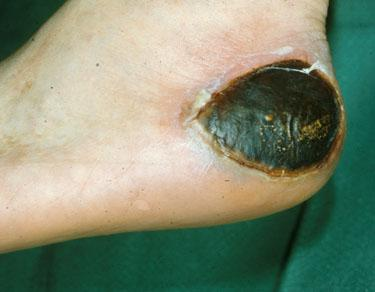
\includegraphics[width=\textwidth]{gambar/gambar-3_2(b).jpg}
		\caption{}
	  \end{subfigure}  
	  \begin{subfigure}{0.3\textwidth}
		\centering{}
		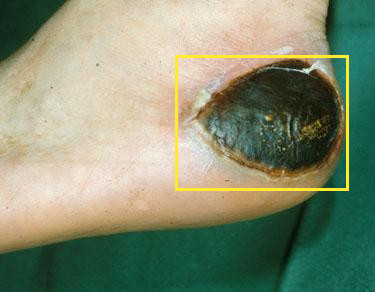
\includegraphics[width=\textwidth]{gambar/rectangle.png}
		\caption{}
	  \end{subfigure}
	\caption{
		(a) Data citra luka 2.png, (b) Inisasi kotak pembatas
        }
  \end{figure}

\subsection{Implementasi Algoritma \emph{GrabCut}}
Setelah kotak tergambar, pada tahap ini terdapat beberapa algoritma yaitu inisiasi 
dan mempelajari \emph{Gaussian Mixture Models} (GMM), dan segmentasi citra \emph{GraphCut}. 
Inisiasi GMM digunakan untuk memperoleh nilai probabilistik dari tiap piksel yang ada
didalam \((T_{U})\). GMM terdiri dari beberapa parameter yaitu \textbf{K} komponen, 
rata-rata \(\mu\), matriks kovarians \(\Sigma\), dan probabilitas prior \(\omega\). 
Selanjutnya mempelajari parameter GMM yang berdasarkan probabilitas dari parameter 
GMM tiap piksel. Setelah mempelajari nilai dari parameter GMM tiap piksel.

Setelah mempelajari parameter GMM dari tiap piksel, maka diperoleh nilai parameter
untuk komponen yang ada pada setiap piksel, masuk ke tahap segmentasi citra luka 
dengan menggunakan algoritma \emph{GraphCut}. Algoritma ini memvisualisasikan tiap piksel 
dari citra sebagai sebuah graf yang saling terhubung, satuan piksel pada gambar bisa
disebut sebagai \emph{node} pada graf yang mana tiap node akan memiliki komponen yang 
berasal dari nilai GMM tadi, pada graf yang sudah terbentuk maka akan ada dua terminal
yaitu terminal \emph{source} dan terminal \emph{sink}, partisi graf (kumpulan \emph{node}) 
yang memiliki hubungan probabilitas ke terminal \emph{source} akan menjadi \emph{foreground}
dan partisi graf yang memiliki hubungan probabilitas ke terminal \emph{sink} akan
menjadi \emph{background}. Algoritma ini memanfaatkan nilai dari GMM yang sudah dipelajari dan \emph{term smoothness}, nilai GMM akan dipakai sebagai
kemungkinan piksel yang termasuk \emph{background} atau \emph{foreground} sedangkan 
\emph{term smoothness} dipakai untuk menghitung hubungan diskontinuitas antar piksel.

\begin{figure}[H]
	\centering{}
	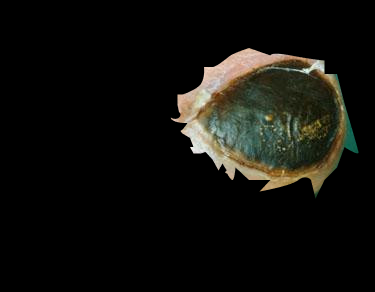
\includegraphics[width=0.4\textwidth]{gambar/res_1.png}
	\caption{Hasil segmentasi dengan \emph{GrabCut} sebelum diperbaiki}
  \end{figure}

\subsection{Penyuntingan oleh Pengguna}
Langkah selanjutnya melakukan perbaikan dari citra yang sudah di segmentasi
dari hasil sebelumnya dengan menetapkan piksel yang seharusnya menjadi latar belakang
atau latar depan dengan melakukan langkah \emph{mincut} yang dilakukan sekali.

\begin{figure}[H]
	\centering
      \begin{subfigure}{0.3\textwidth}
		\centering{}
		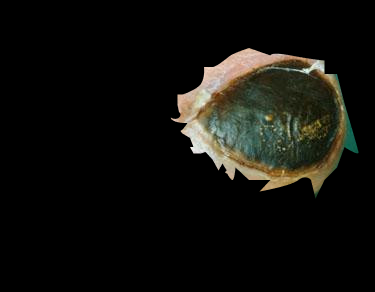
\includegraphics[width=\textwidth]{gambar/res_1.png}
		\caption{}
	  \end{subfigure}
      \begin{subfigure}{0.3\textwidth}
		\centering{}
		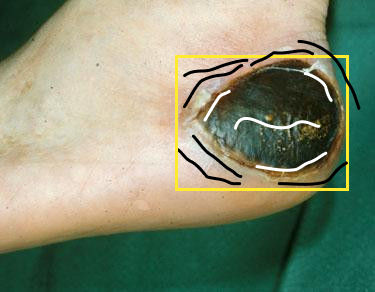
\includegraphics[width=\textwidth]{gambar/brush.png}
		\caption{}
	  \end{subfigure}
      \begin{subfigure}{0.3\textwidth}
		\centering{}
		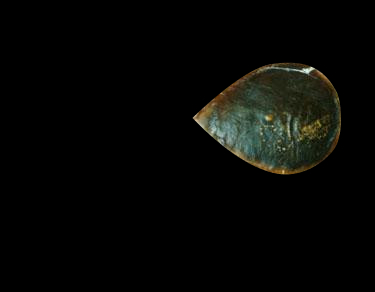
\includegraphics[width=\textwidth]{gambar/res_2.png}
		\caption{}
	  \end{subfigure}
	\caption{
		(a) Hasil \emph{Grabcut} sebelum diperbaiki, (b) Penyuntingan oleh pengguna, (c) Hasil 
        segmentasi \emph{GrabCut} setelah diperbaiki
	 }
  \end{figure}

\section{Diagram Alir Segmentasi Luka dengan Metode \emph{GrabCut}}
Berikut adalah diagram alir segmentasi luka dengan metode \emph{GrabCut}: 
\begin{figure}[H]
	\centering{}
	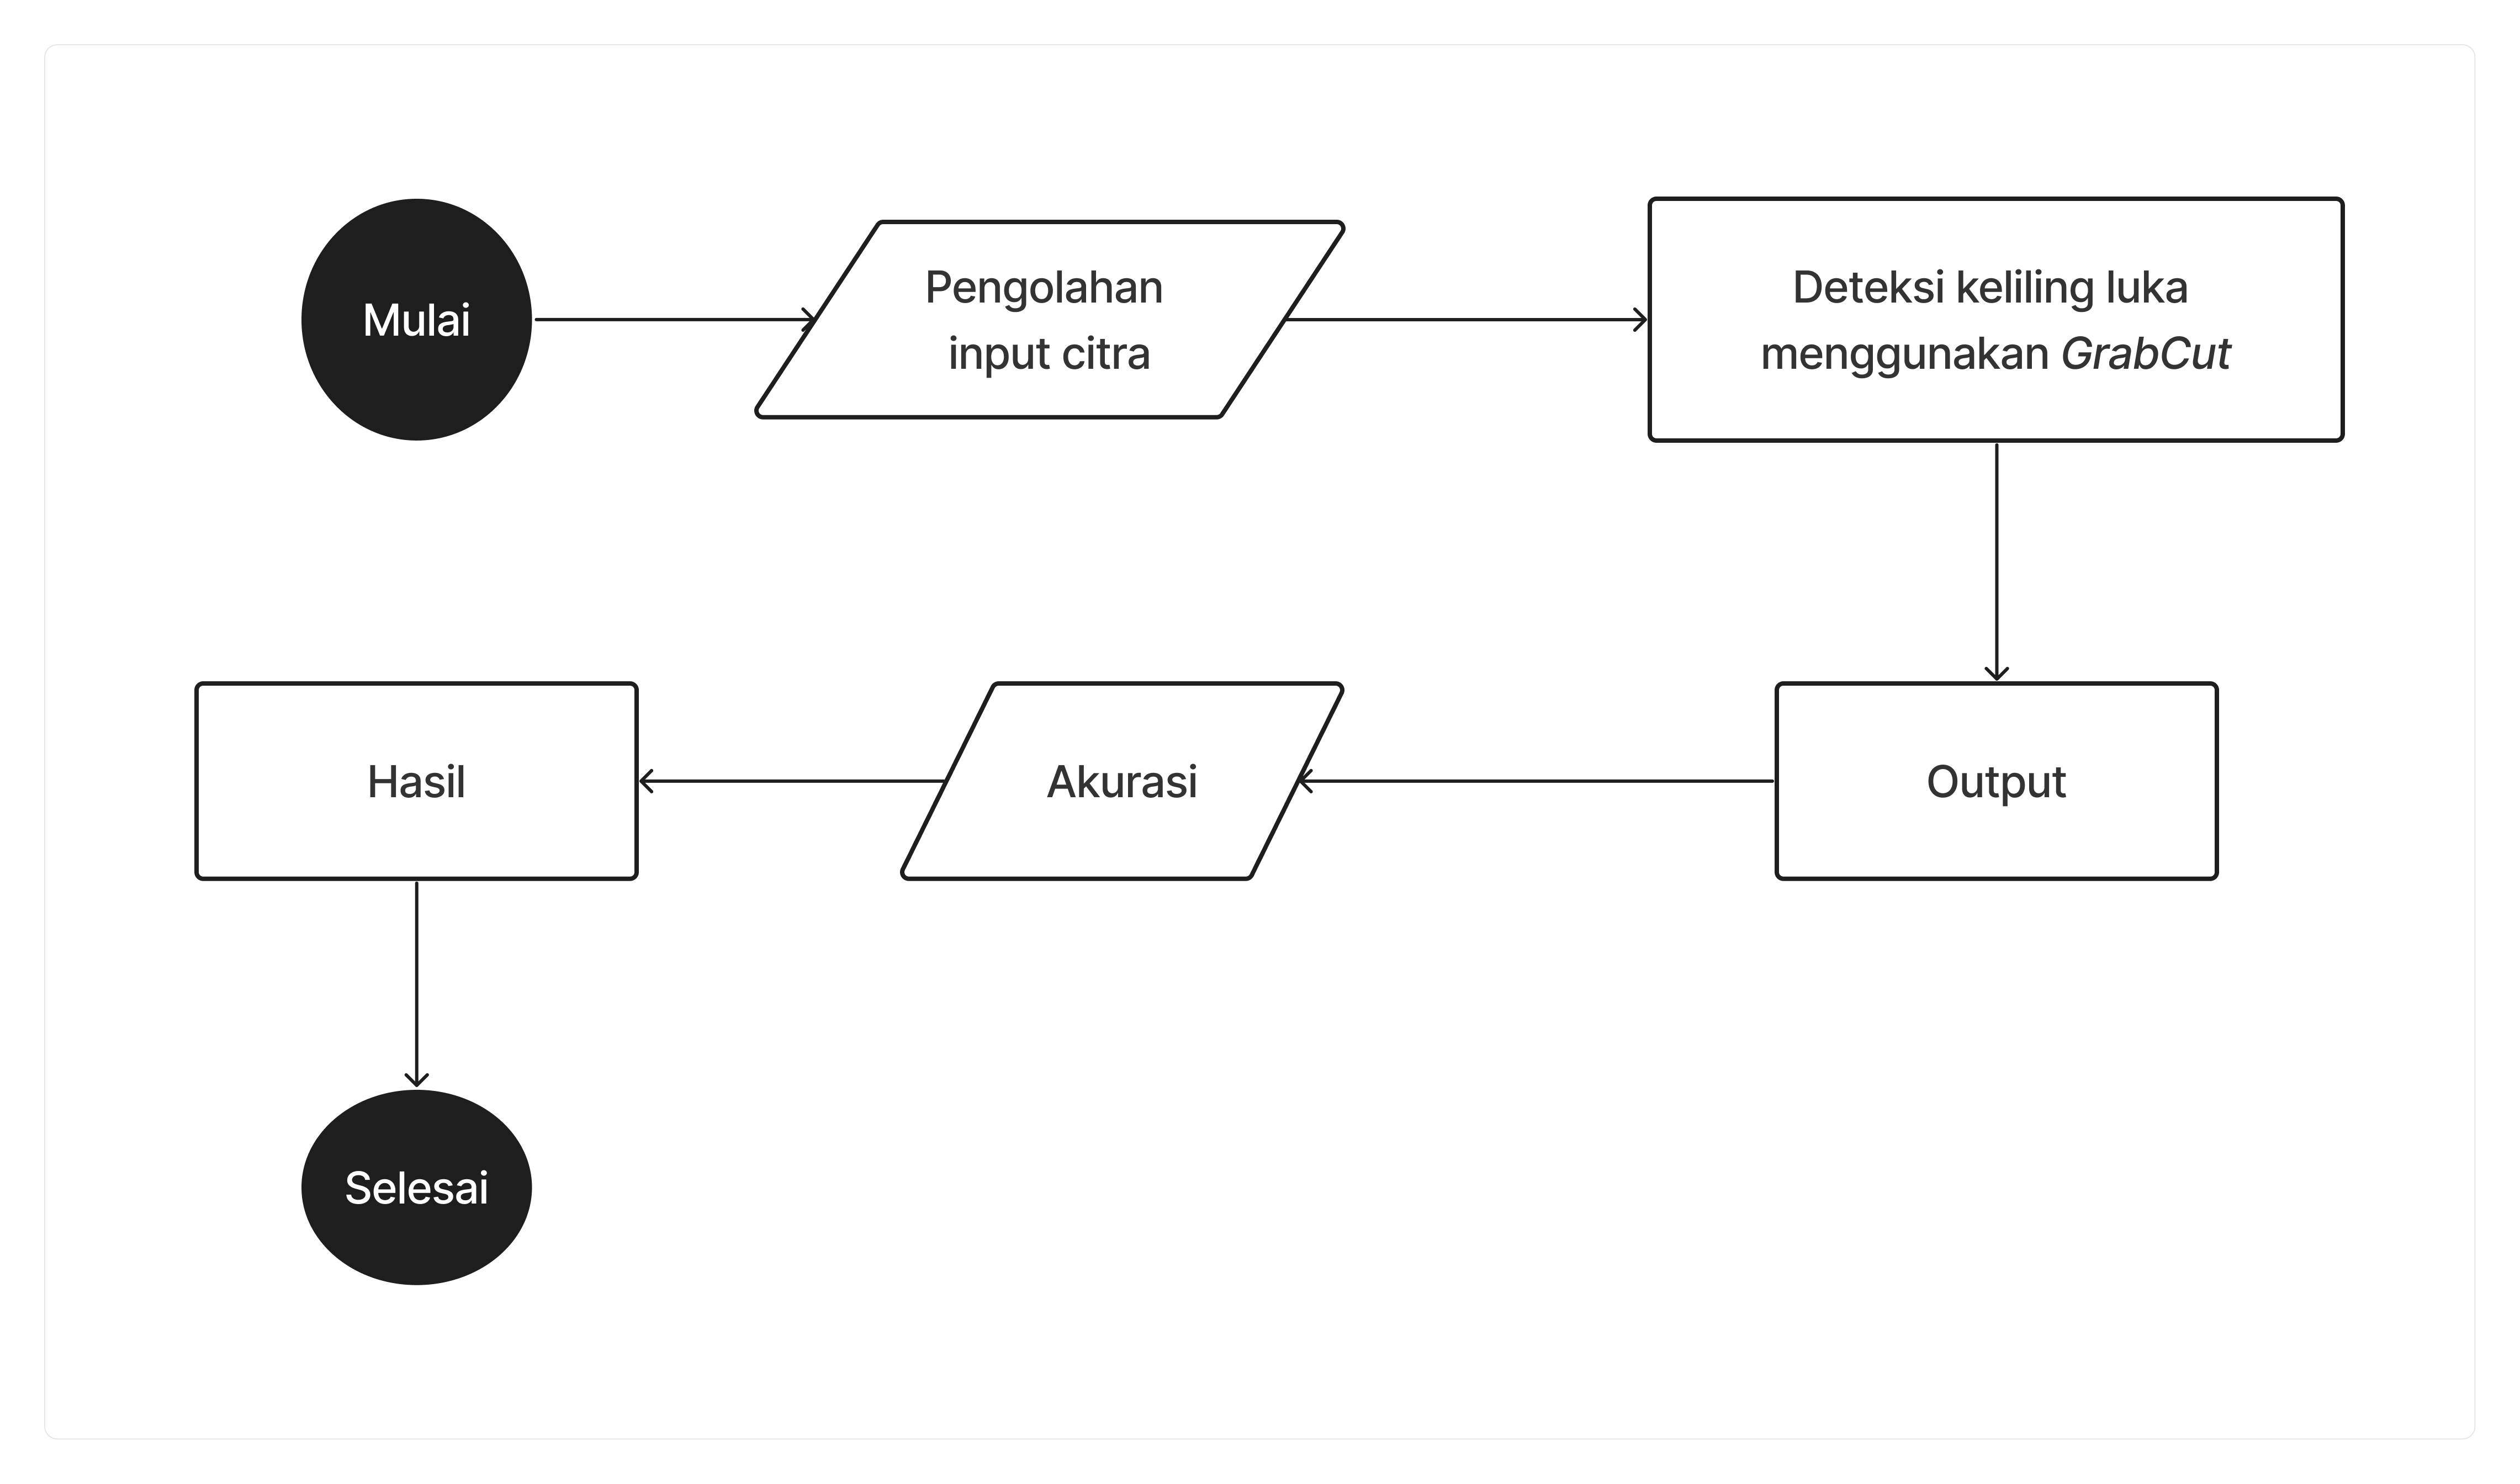
\includegraphics[width=0.8\textwidth]{gambar/diagram_penelitian.png}
	\caption{Diagram alir penelitian}
	\label{img:diagram_penelitian}
  \end{figure}

\begin{figure}[H]
	\centering{}
	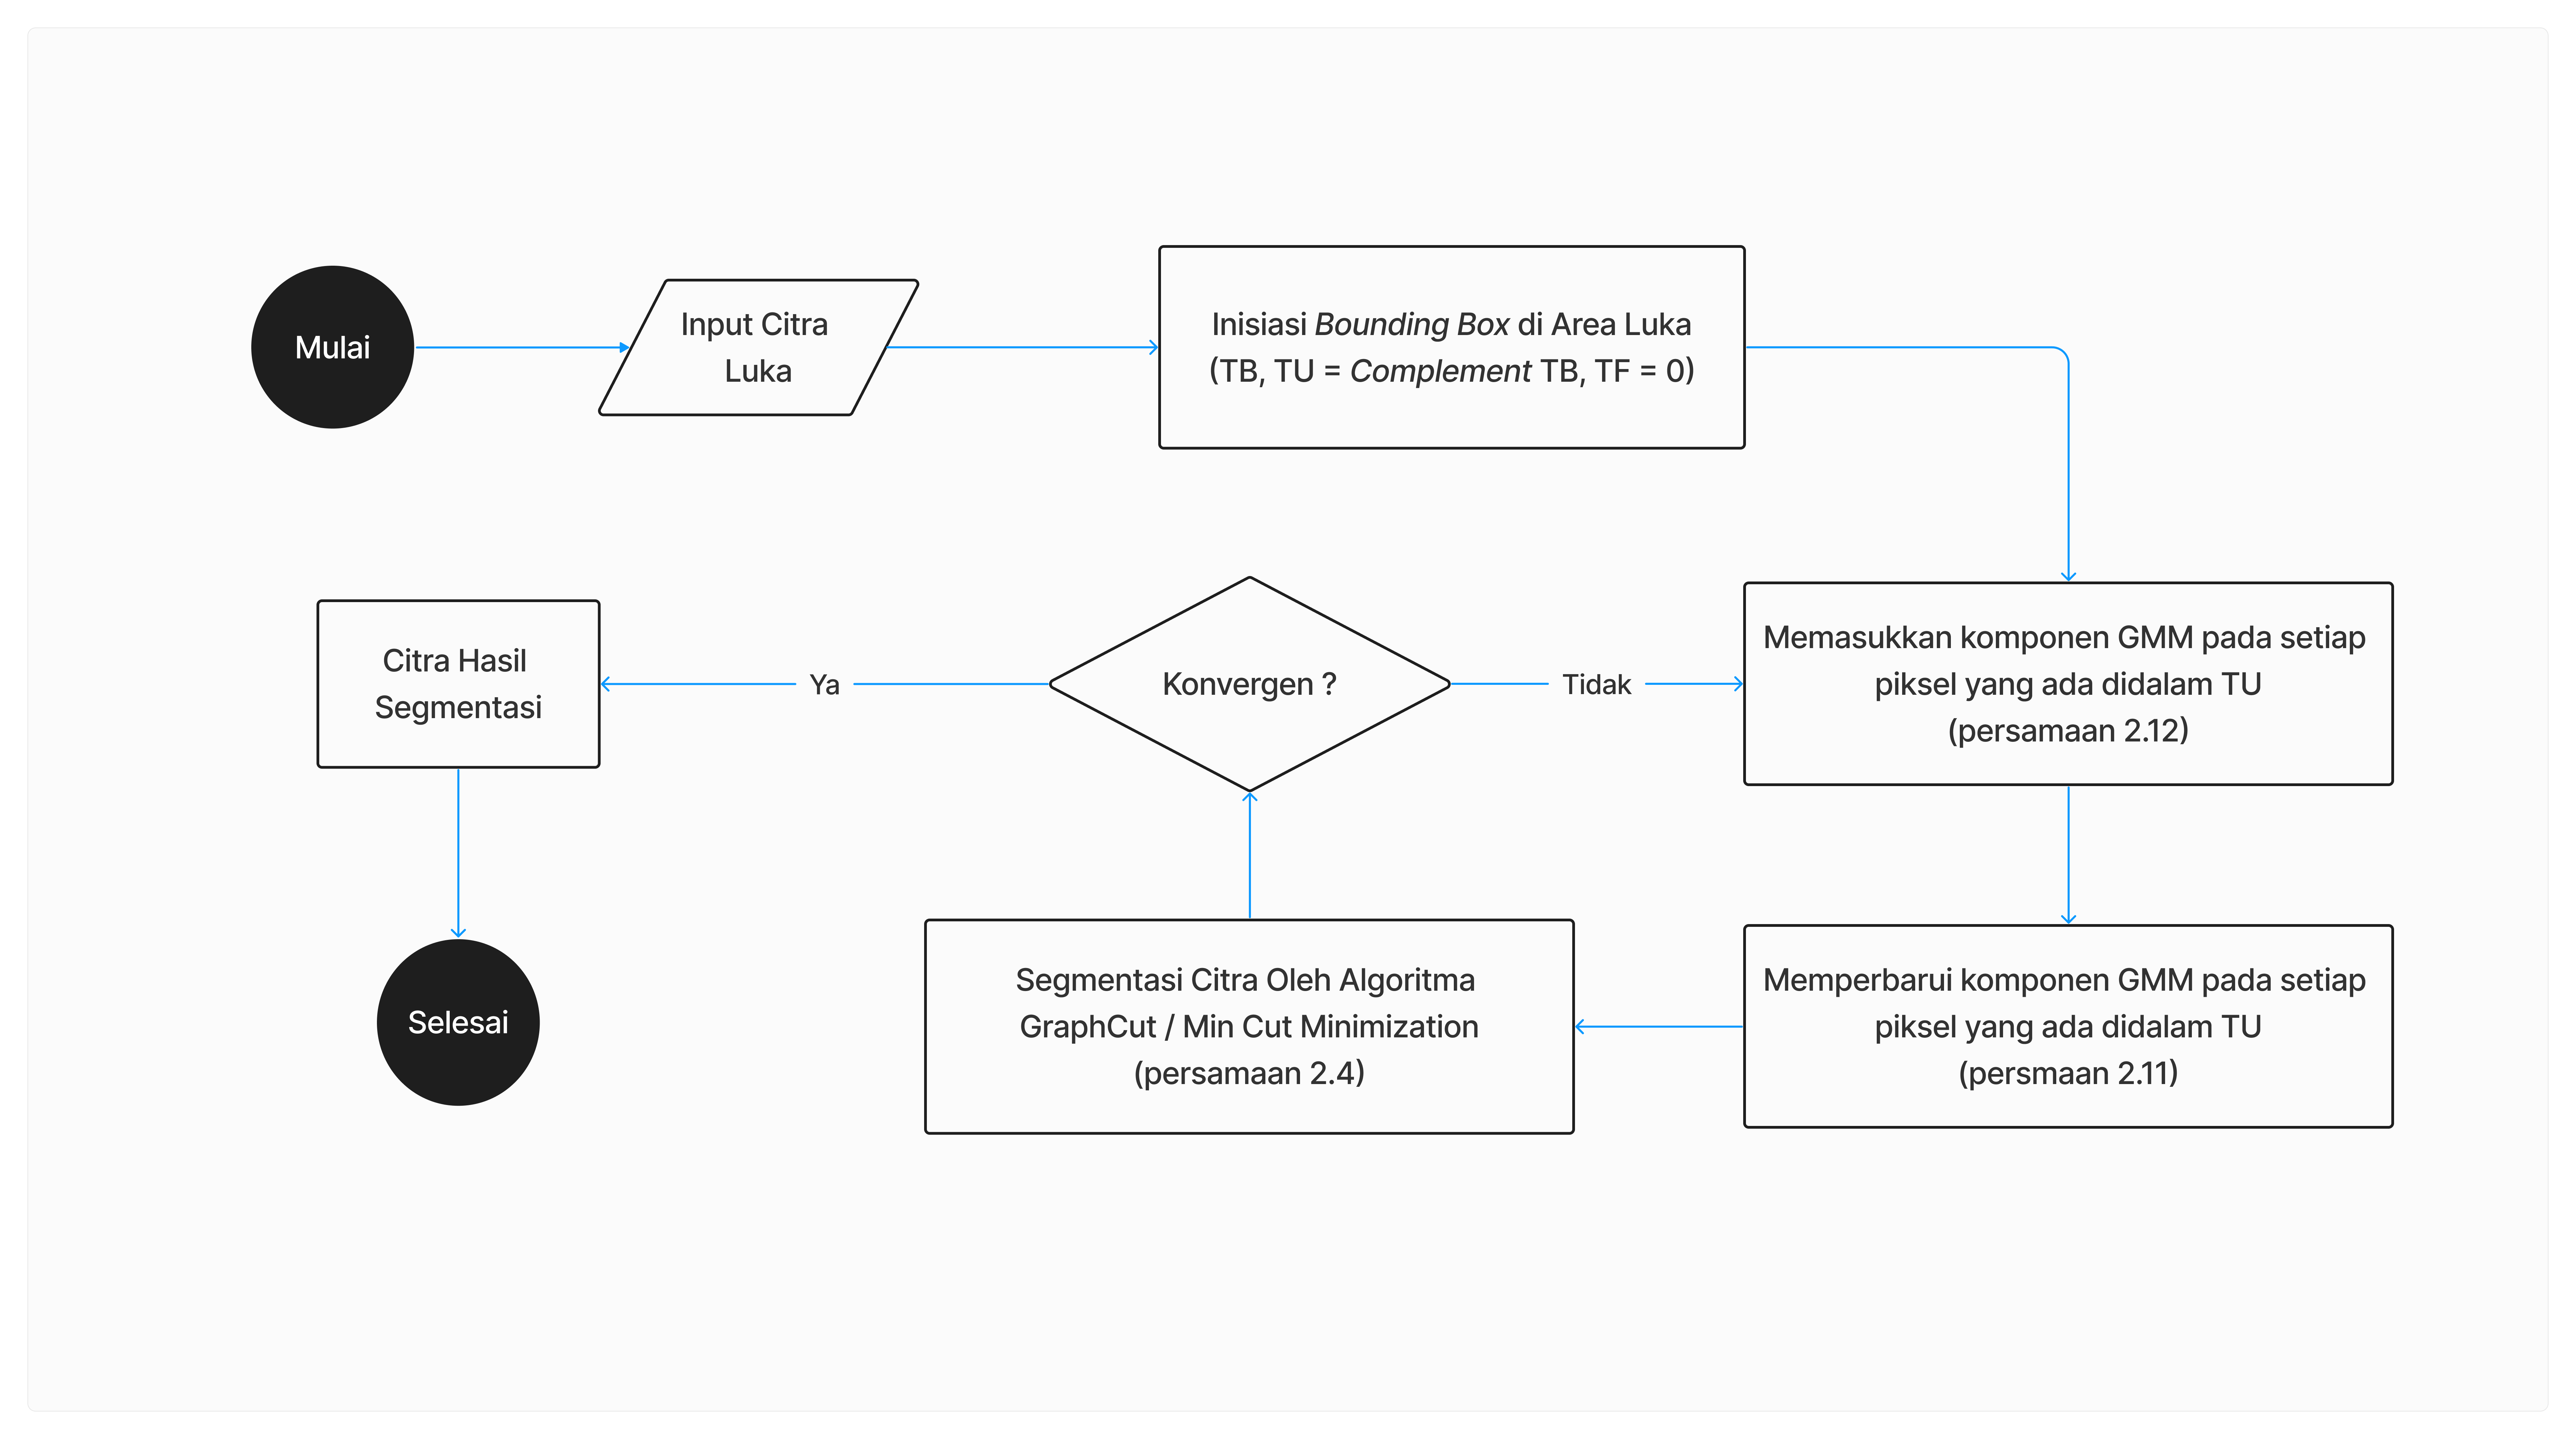
\includegraphics[width=0.9\textwidth]{gambar/diagram_grabcut.png}
	\caption{Diagram alir metode \emph{GrabCut}}
  \end{figure}

\begin{figure}[H]
	\centering{}
	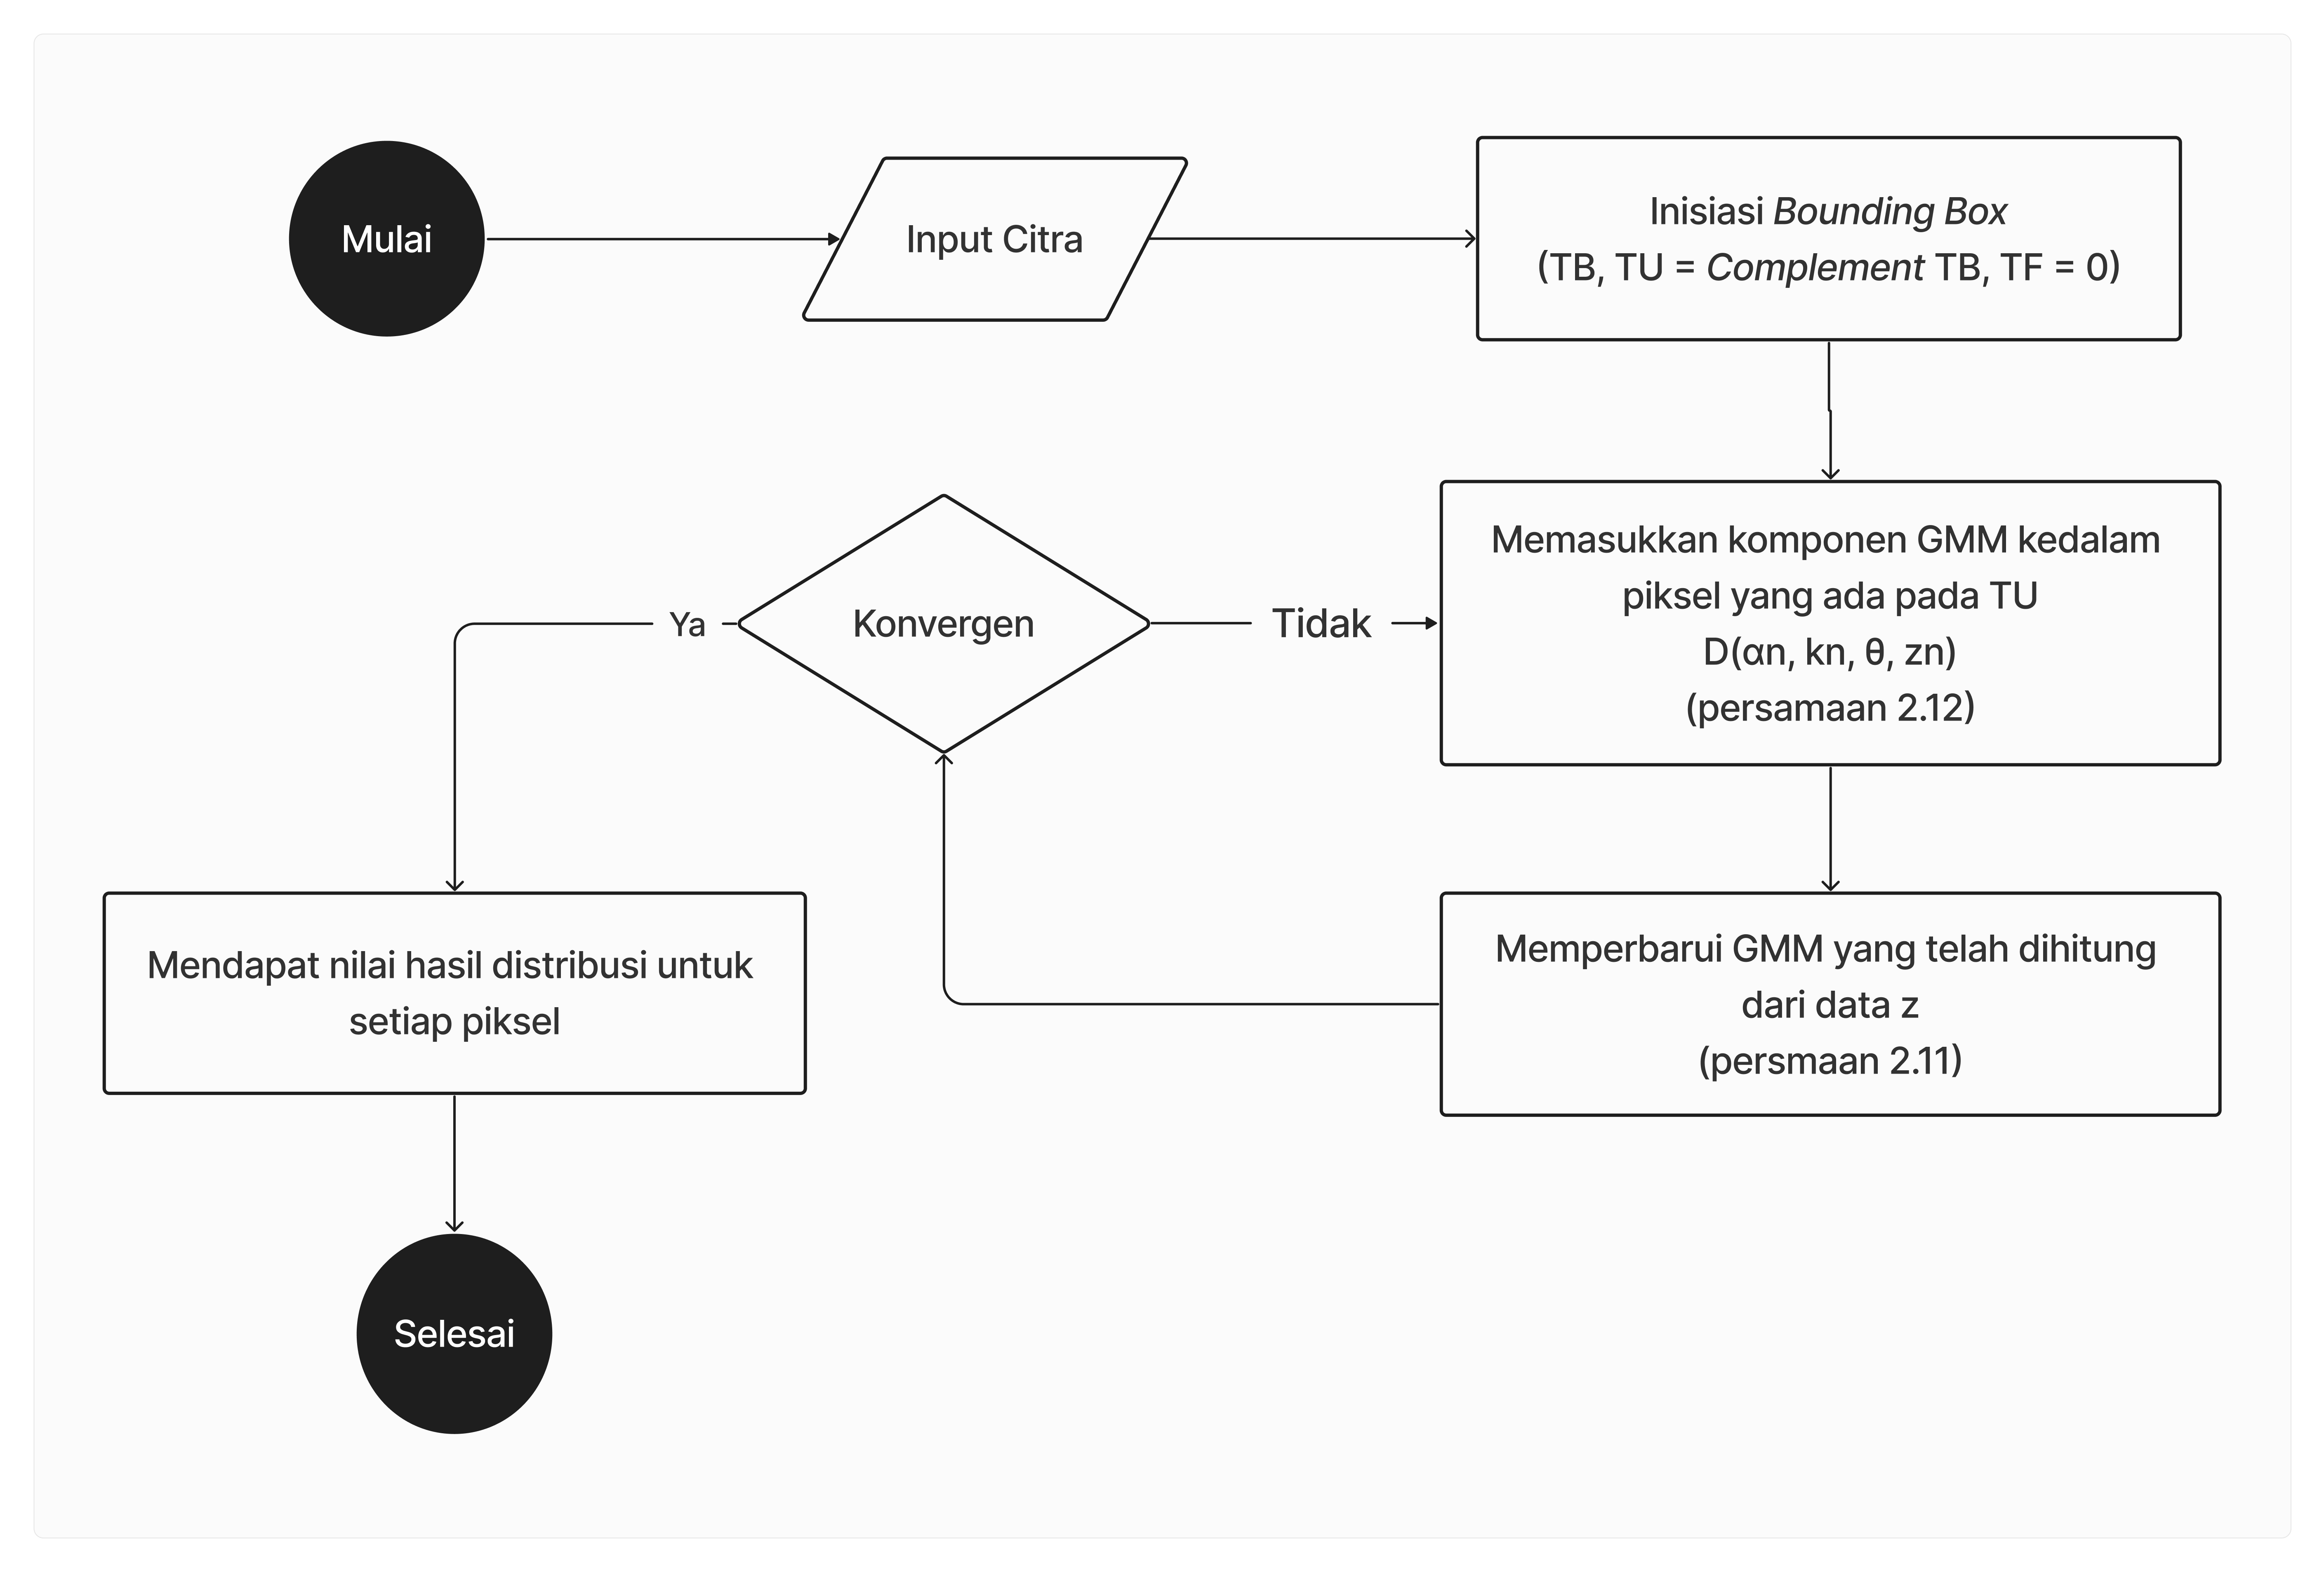
\includegraphics[width=0.9\textwidth]{gambar/diagram_gmm.png}
	\caption{Diagram alir tahap \emph{Gaussian Mixture Models}}
  \end{figure}

\section{Struktur Data}

\subsection{\emph{Node}}

\emph{Node} merupakan elemen dasar dalam pembentukan struktur data seperti \emph{linked list},
pohon, dan graf. Sebuah \emph{node} setidaknya terdiri dari dua komponen, yaitu 
data atau nilai dari \emph{node} tersebut dan referensi atau tautan yang menghubungkan 
\emph{node} tersebut dengan \emph{node} lainnya. Penulis menggunakan struktur data \emph{node} untuk merepresentasikan piksel dari
citra luka, setiap piksel dari gambar menyimpan beberapa informasi, di antaranya komponen warna
RGB (\emph{Red,Green,Blue}), komponen GMM dan nilai label piksel.

\begin{figure}[H]
	\centering{}
	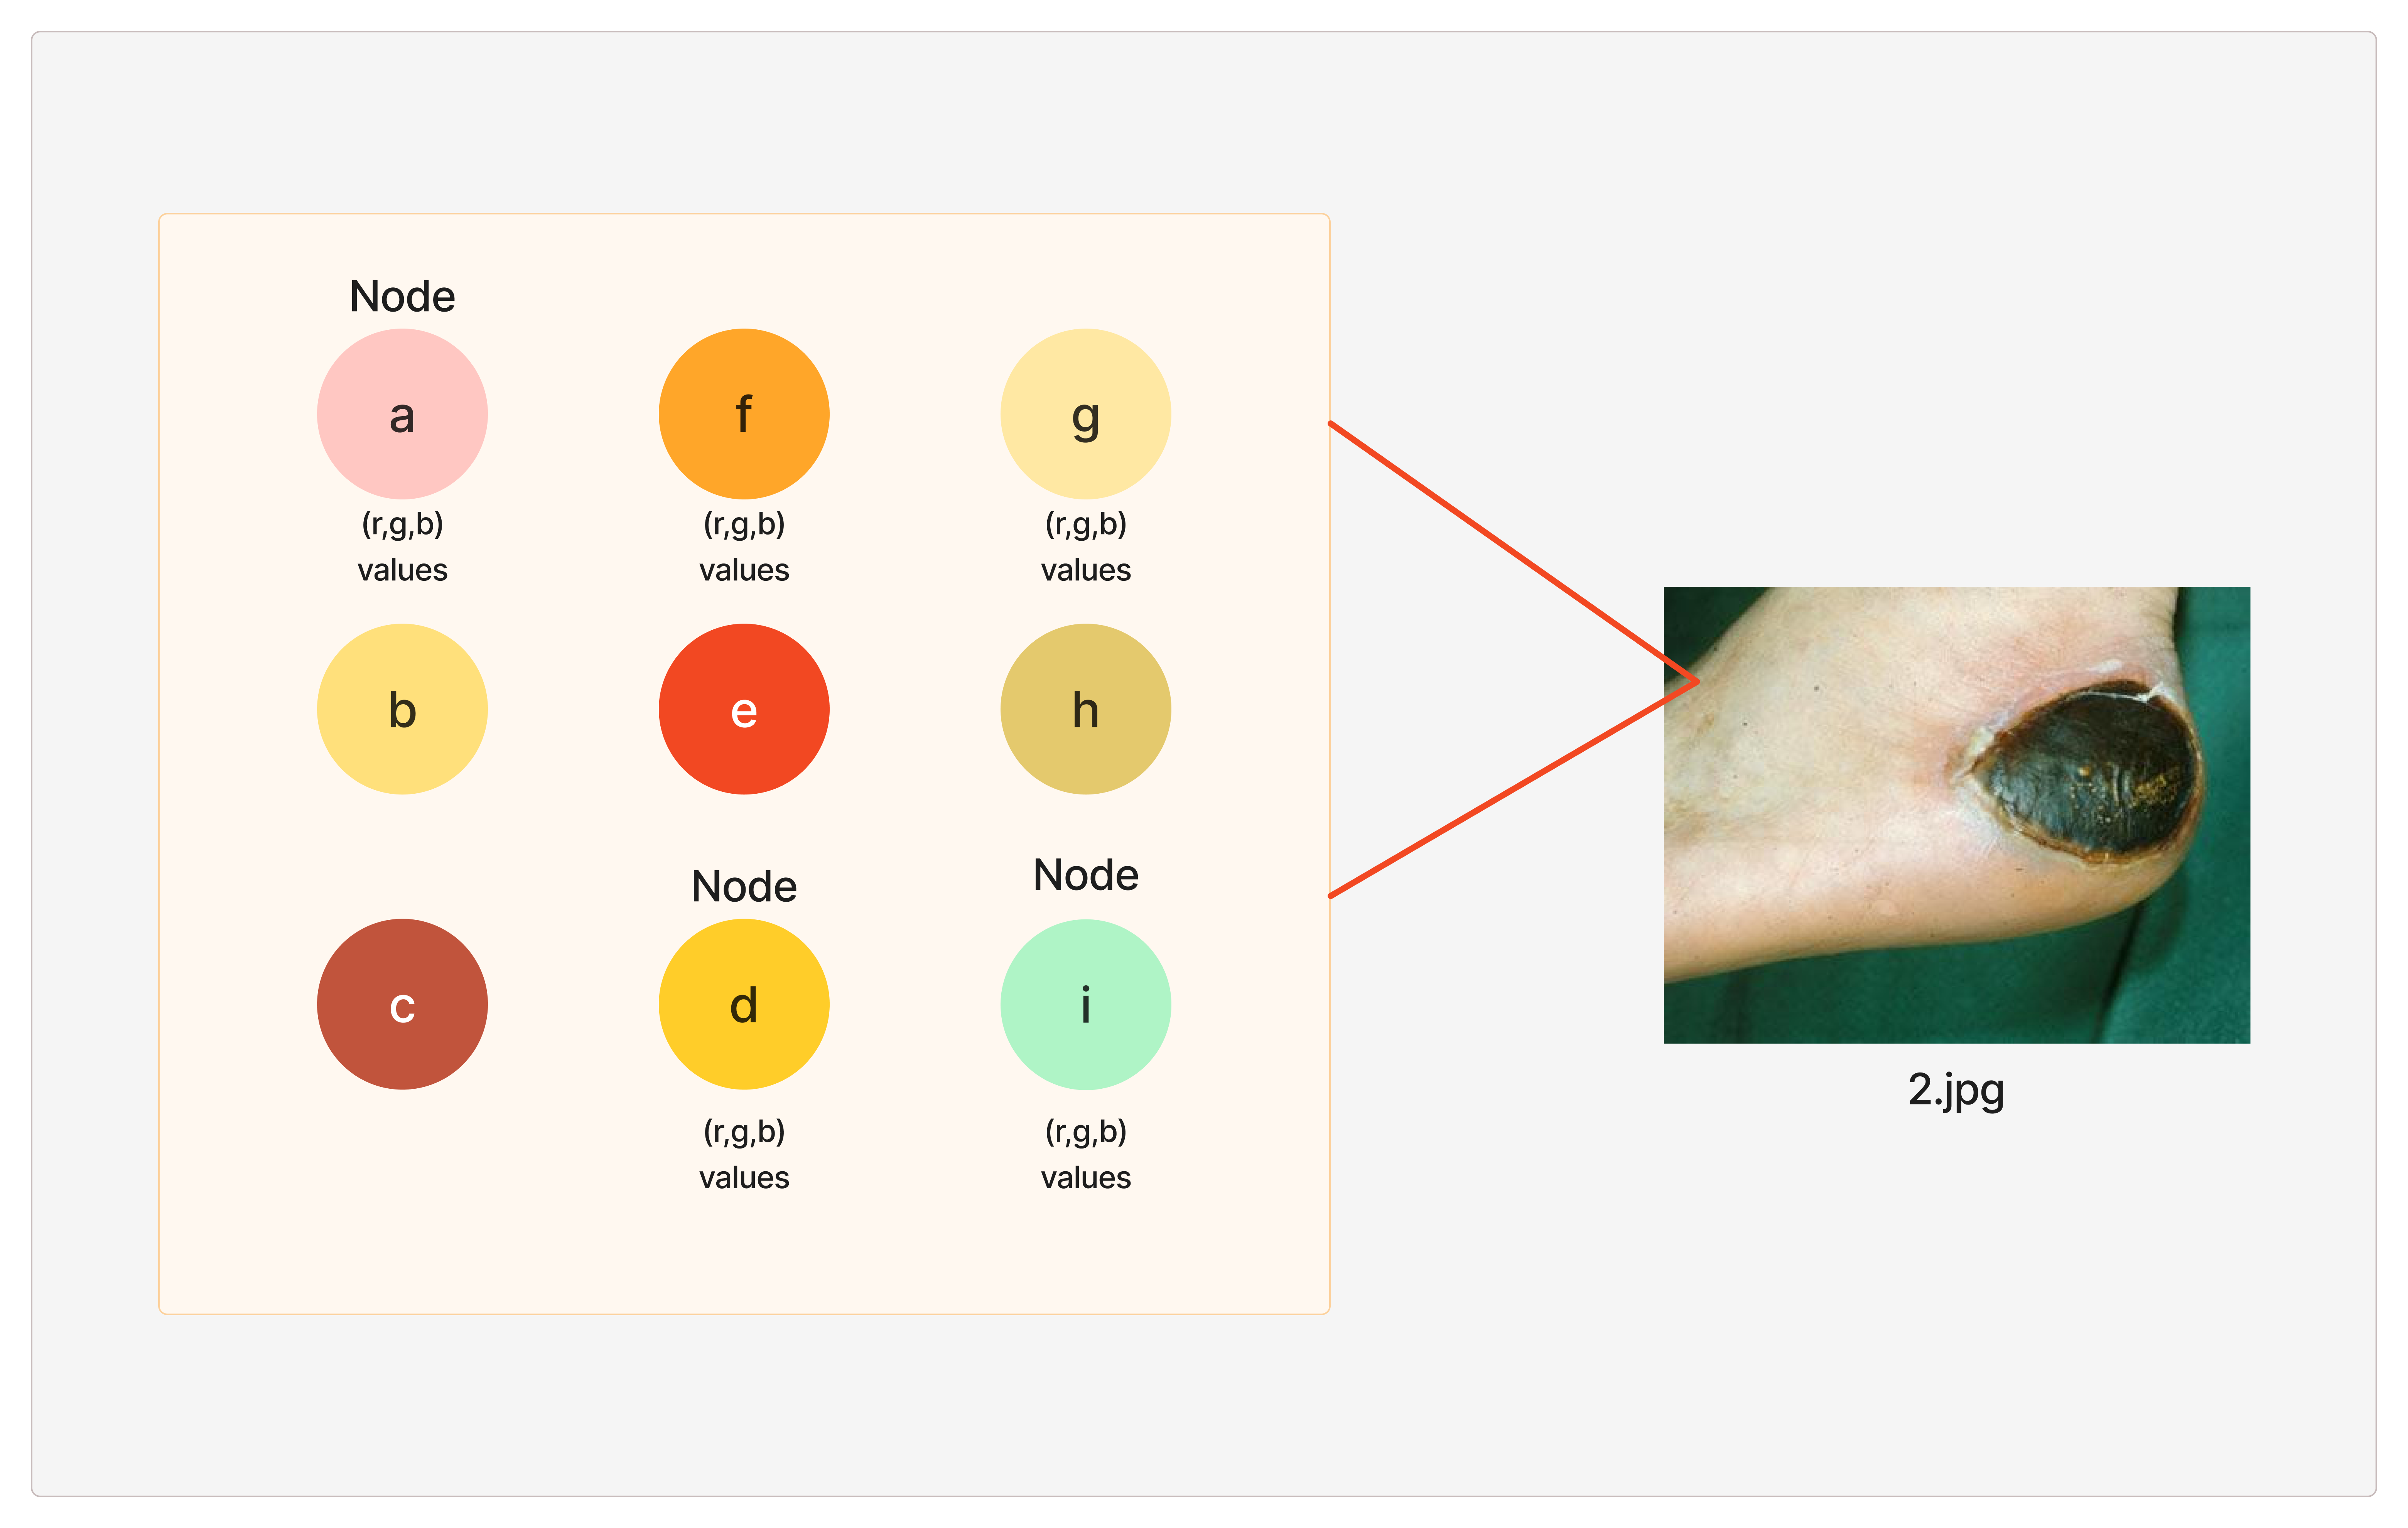
\includegraphics[width=0.5\textwidth]{gambar/node_representasi.png}
	\caption{Representasi \emph{node} terhadap piksel pada gambar}
\end{figure}

Tiap informasi yang ada pada \emph{node} akan dipergunakan dalam algoritma \emph{mincut}
dengan struktur data sebagai berikut :

\begin{lstlisting} [language=C++, caption=Struktur data \emph{node}]
// Struktur Data Node dari piksel
class Node {
    public:
        bool isForeground;
        double foregroundProbability;
        double backgroundProbability;
        vector<GaussianComponent> gmmComponents;
}  
\end{lstlisting}

\subsection{\emph{Linkedlist}} 
Secara umum komponen yang ada \emph{node} di antaranya data yang disimpan dan 
referensi kepada \emph{node} selanjutnya, \emph{linkedlist} akan terbentuk 
dari rangkaian \emph{node} yang saling terhubung.

\begin{figure}[H]
	\centering{}
	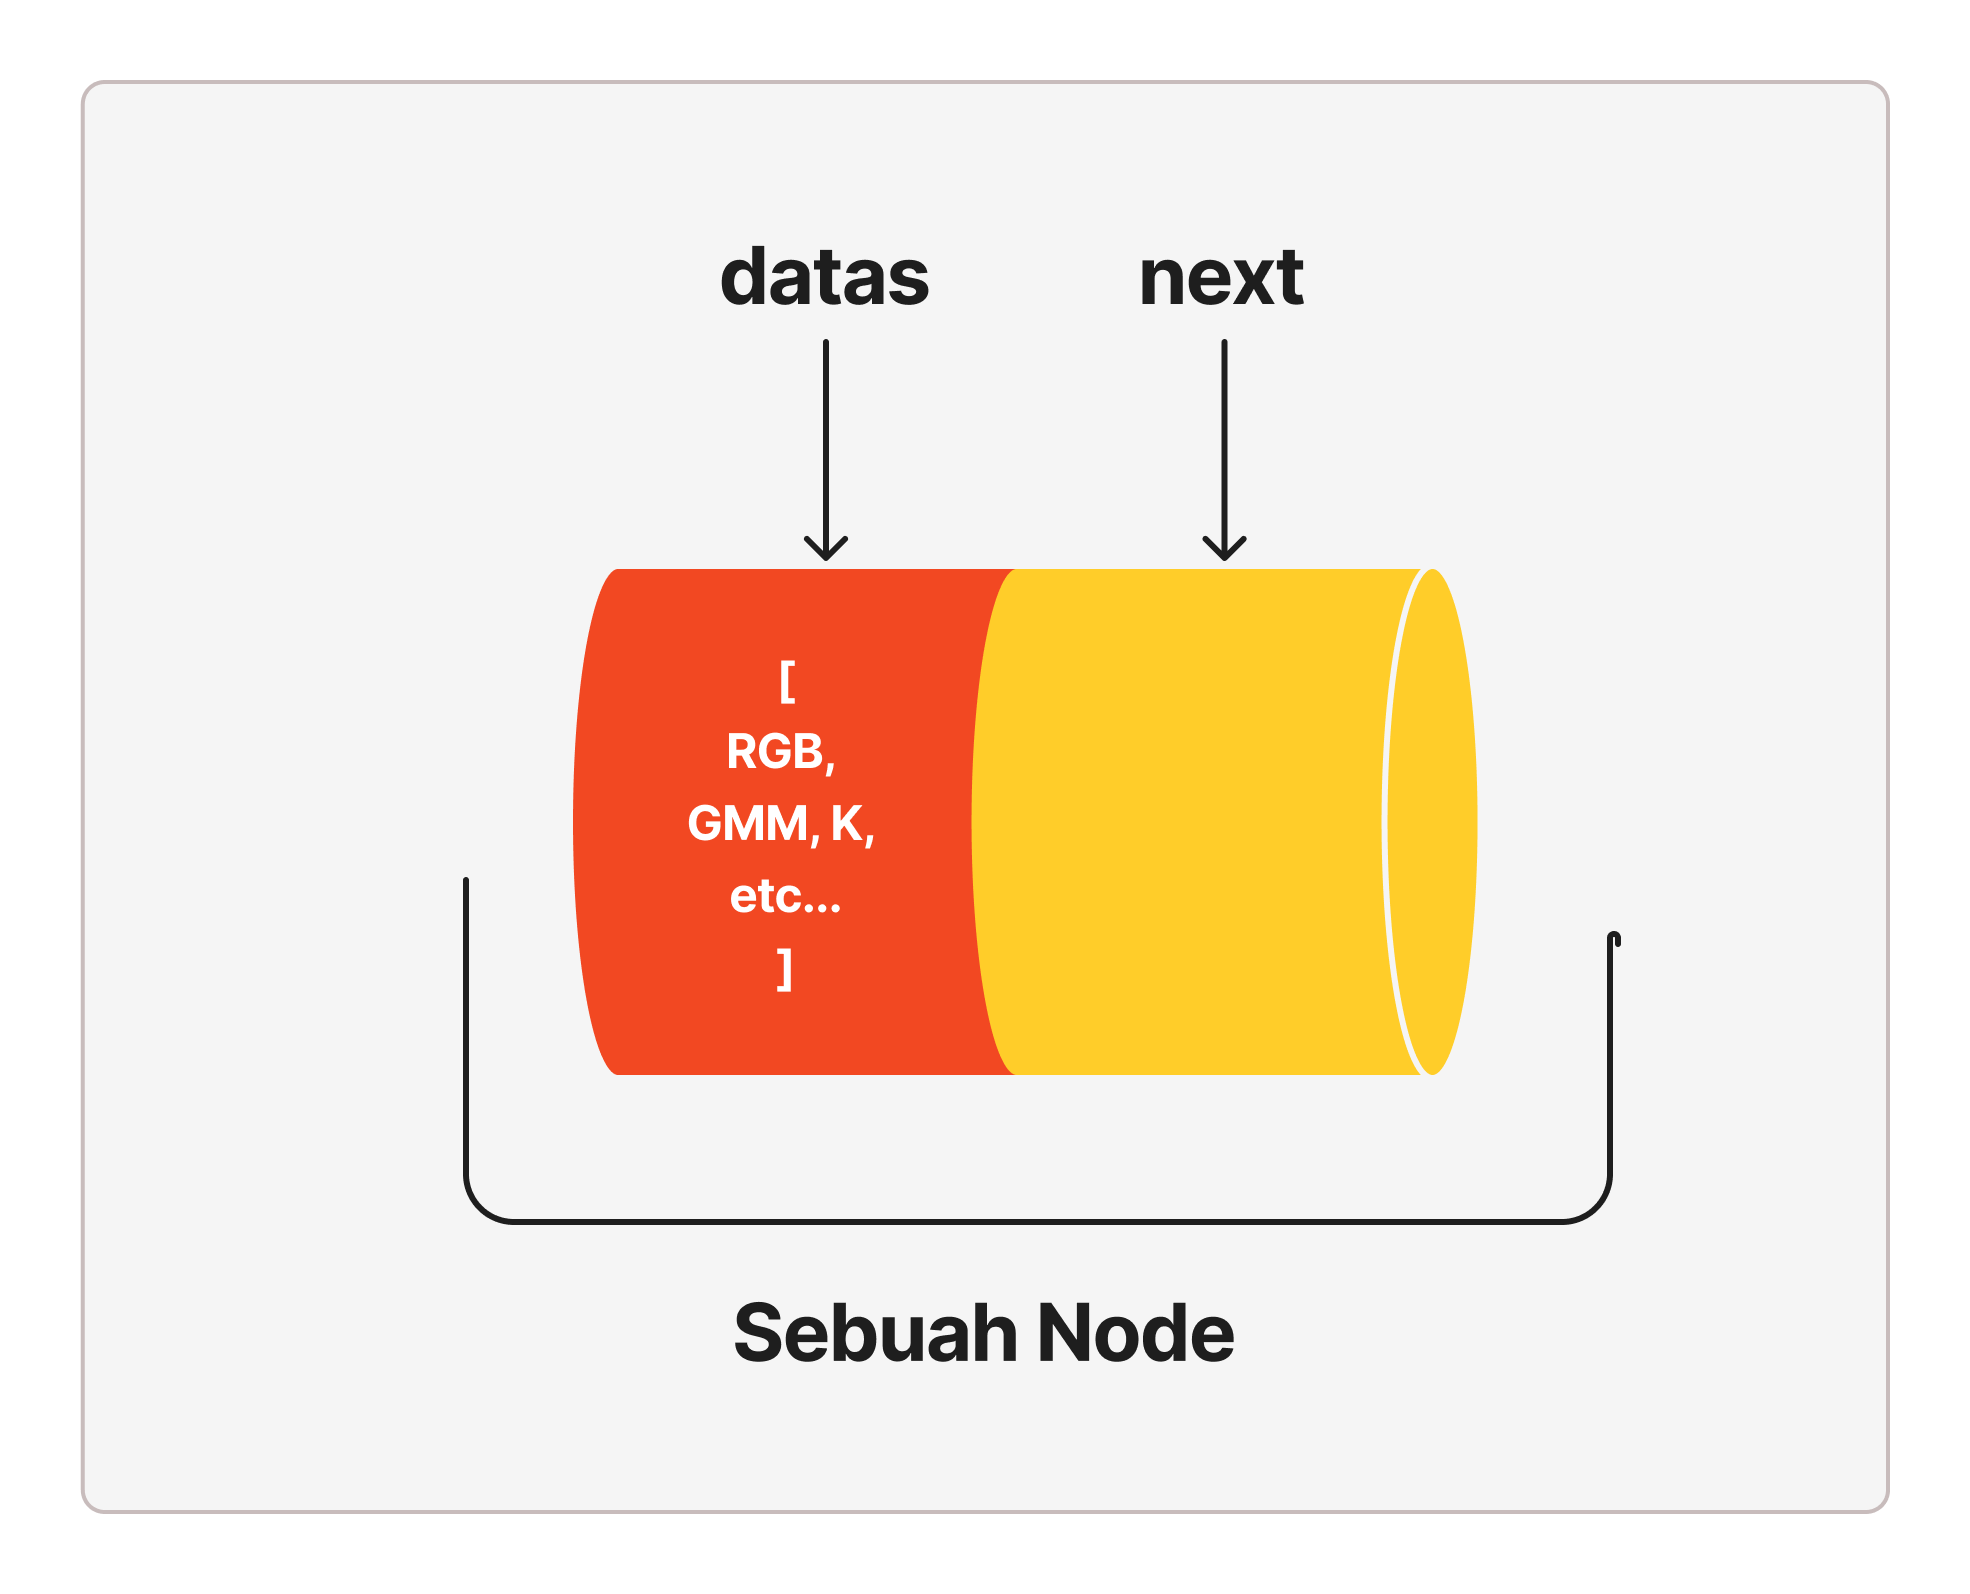
\includegraphics[width=0.6\textwidth]{gambar/node_komponen.png}
	\caption{Komponen yang ada pada sebuah \emph{node}}
\end{figure}

Pada penelitian ini struktur komponen \emph{node} yang akan penulis gunakan 
memiliki tiga komponen itu referensi ke \emph{node} sebelumnya, data dari \emph{node},
dan referensi ke \emph{node} selanjutnya.

\begin{figure}[H]
	\centering{}
	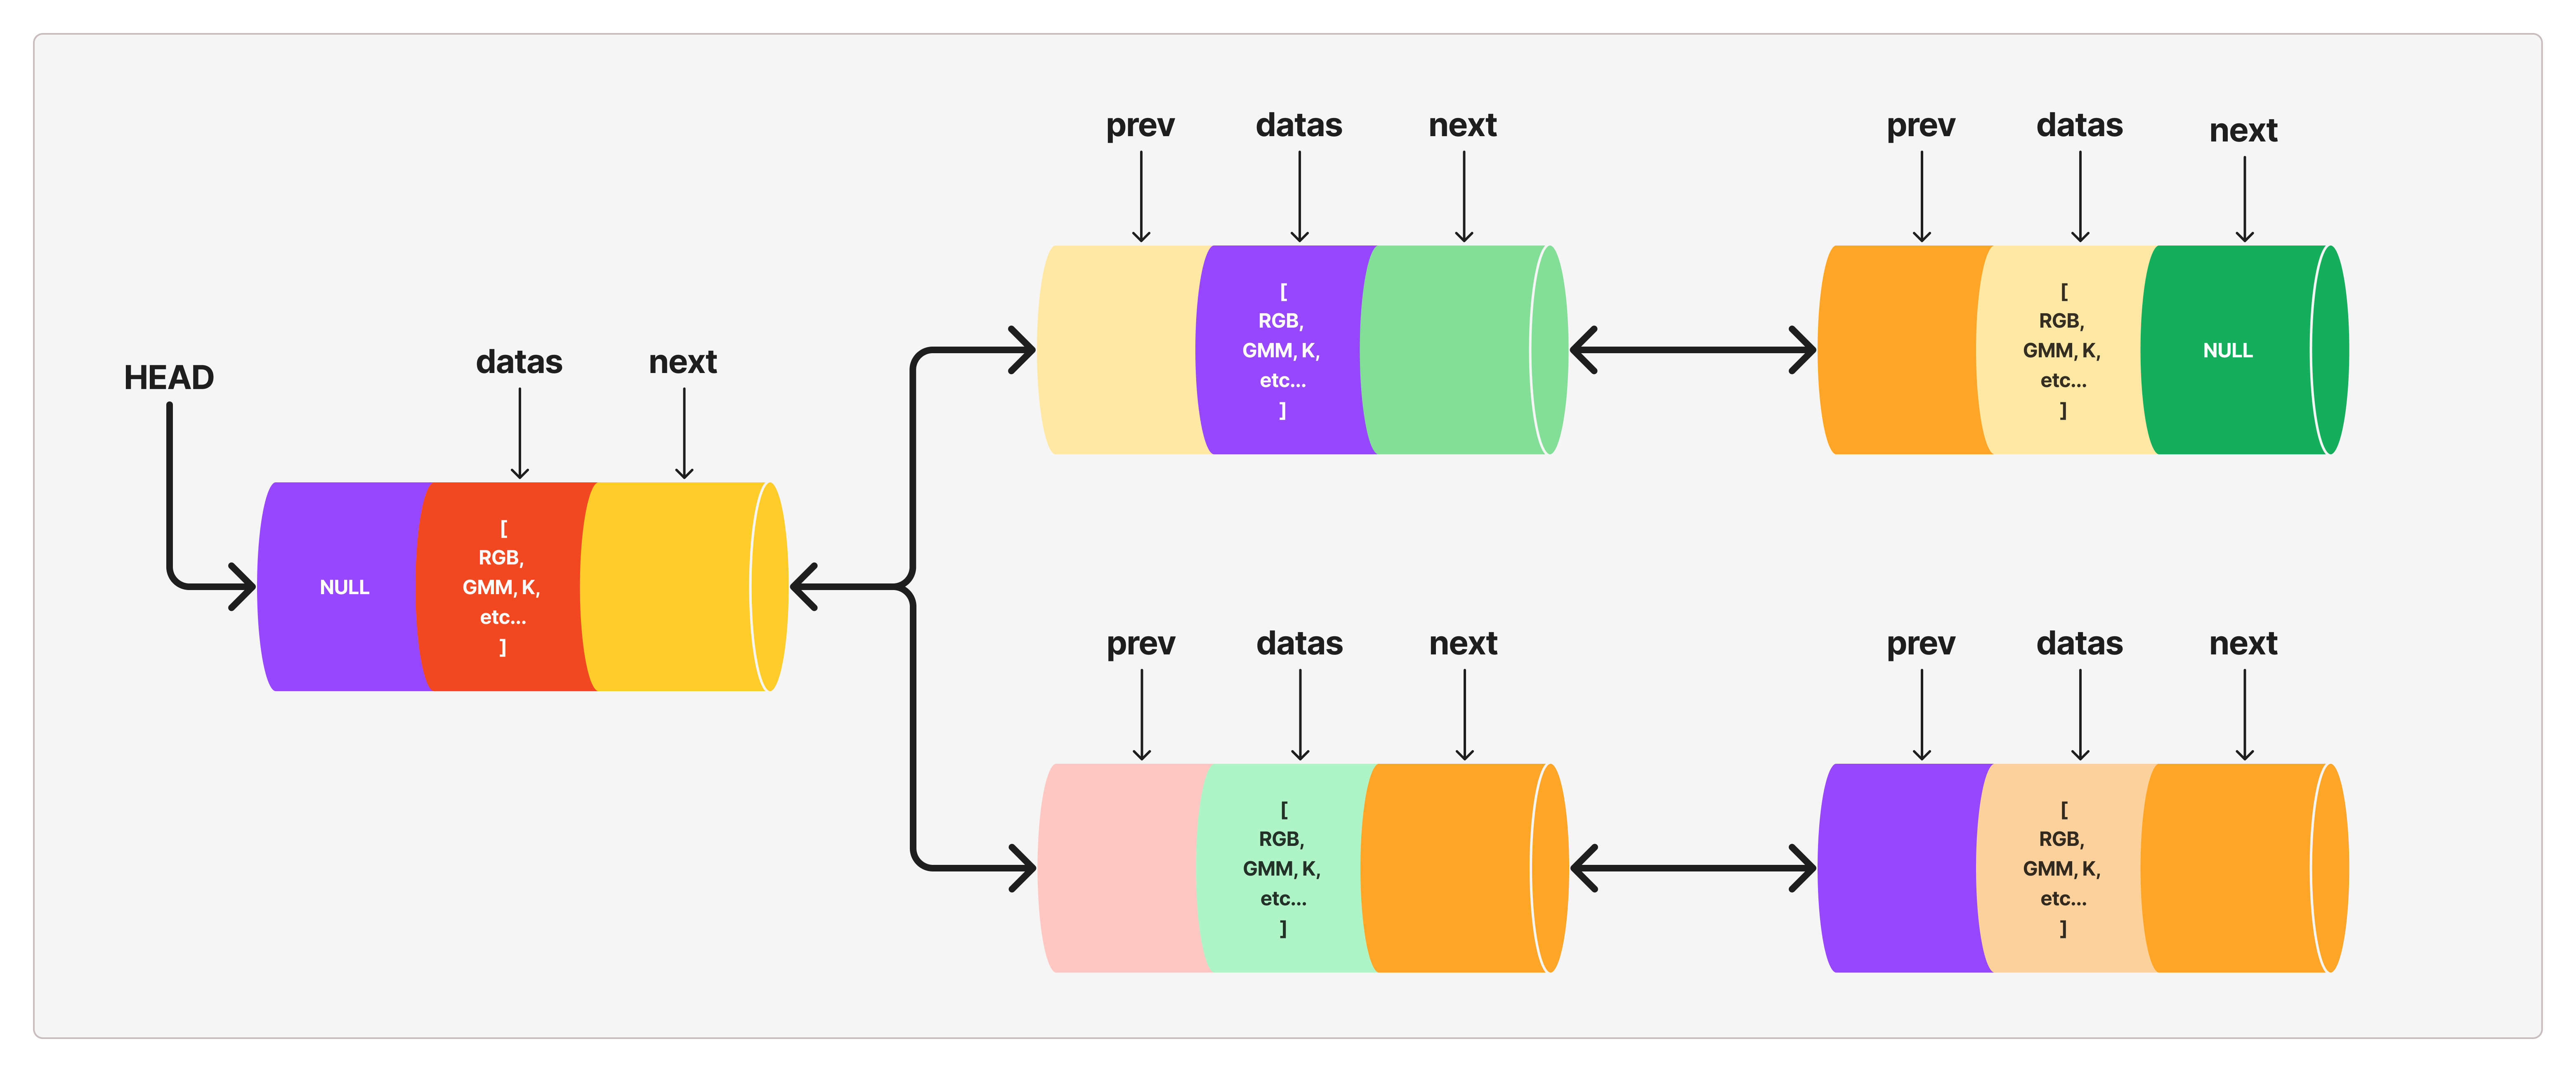
\includegraphics[width=\textwidth]{gambar/linkedlist_example.png}
	\caption{\emph{Linkedlist} terdiri dari susunan \emph{node}}
\end{figure}

Referensi pada \emph{node} bertujuan untuk mengetahui \emph{node} mana yang 
menjadi \emph{parent} menggunakan referensi ke \emph{node} sebelumnya  dan 
\emph{child} menggunakan referensi ke \emph{node} selanjutnya. \emph{Node} yang berada di awal graf akan menjadi \emph{head} dan \emph{node}
terakhir akan ditetapkan sebagai \emph{tail}, sementara komponen data-data
\emph{node} akan disimpan sebagai karakteristik dari \emph{node} tersebut.

\begin{lstlisting} [language=C++, caption=Struktur data \emph{doubly linkedlist}]
// Struktur Data LinkedList
class Node {
public:
    bool isForeground;
    double foregroundProbability;
    double backgroundProbability;
    vector<GaussianComponent> gmmComponents;

    Node* parent;
    vector<Node*> children;

    Node(bool isForeground, 
            double foregroundProbability, 
            double backgroundProbability ) {

        this->isForeground = isForeground;
        this->foregroundProbability = 
        foregroundProbability;
        this->backgroundProbability = 
        backgroundProbability;
        
        this->parent = nullptr;
    }
 	}
\end{lstlisting}


\subsection{\emph{Tree}}
Struktur data \emph{tree} merupakan suatu struktur data hirarki, \emph{tree} diibaratkan
sebagai hubungan induk dan anak dalam sebuah pohon, \emph{node} paling atas dari 
\emph{tree} disebut dengan akar (\emph{root}), dan \emph{node} turunannya disebut 
sebagai anak dari \emph{node} lain atau menjadi daun (\emph{node} yang tidak memiliki 
anak)
\begin{figure}[H]
	\centering{}
	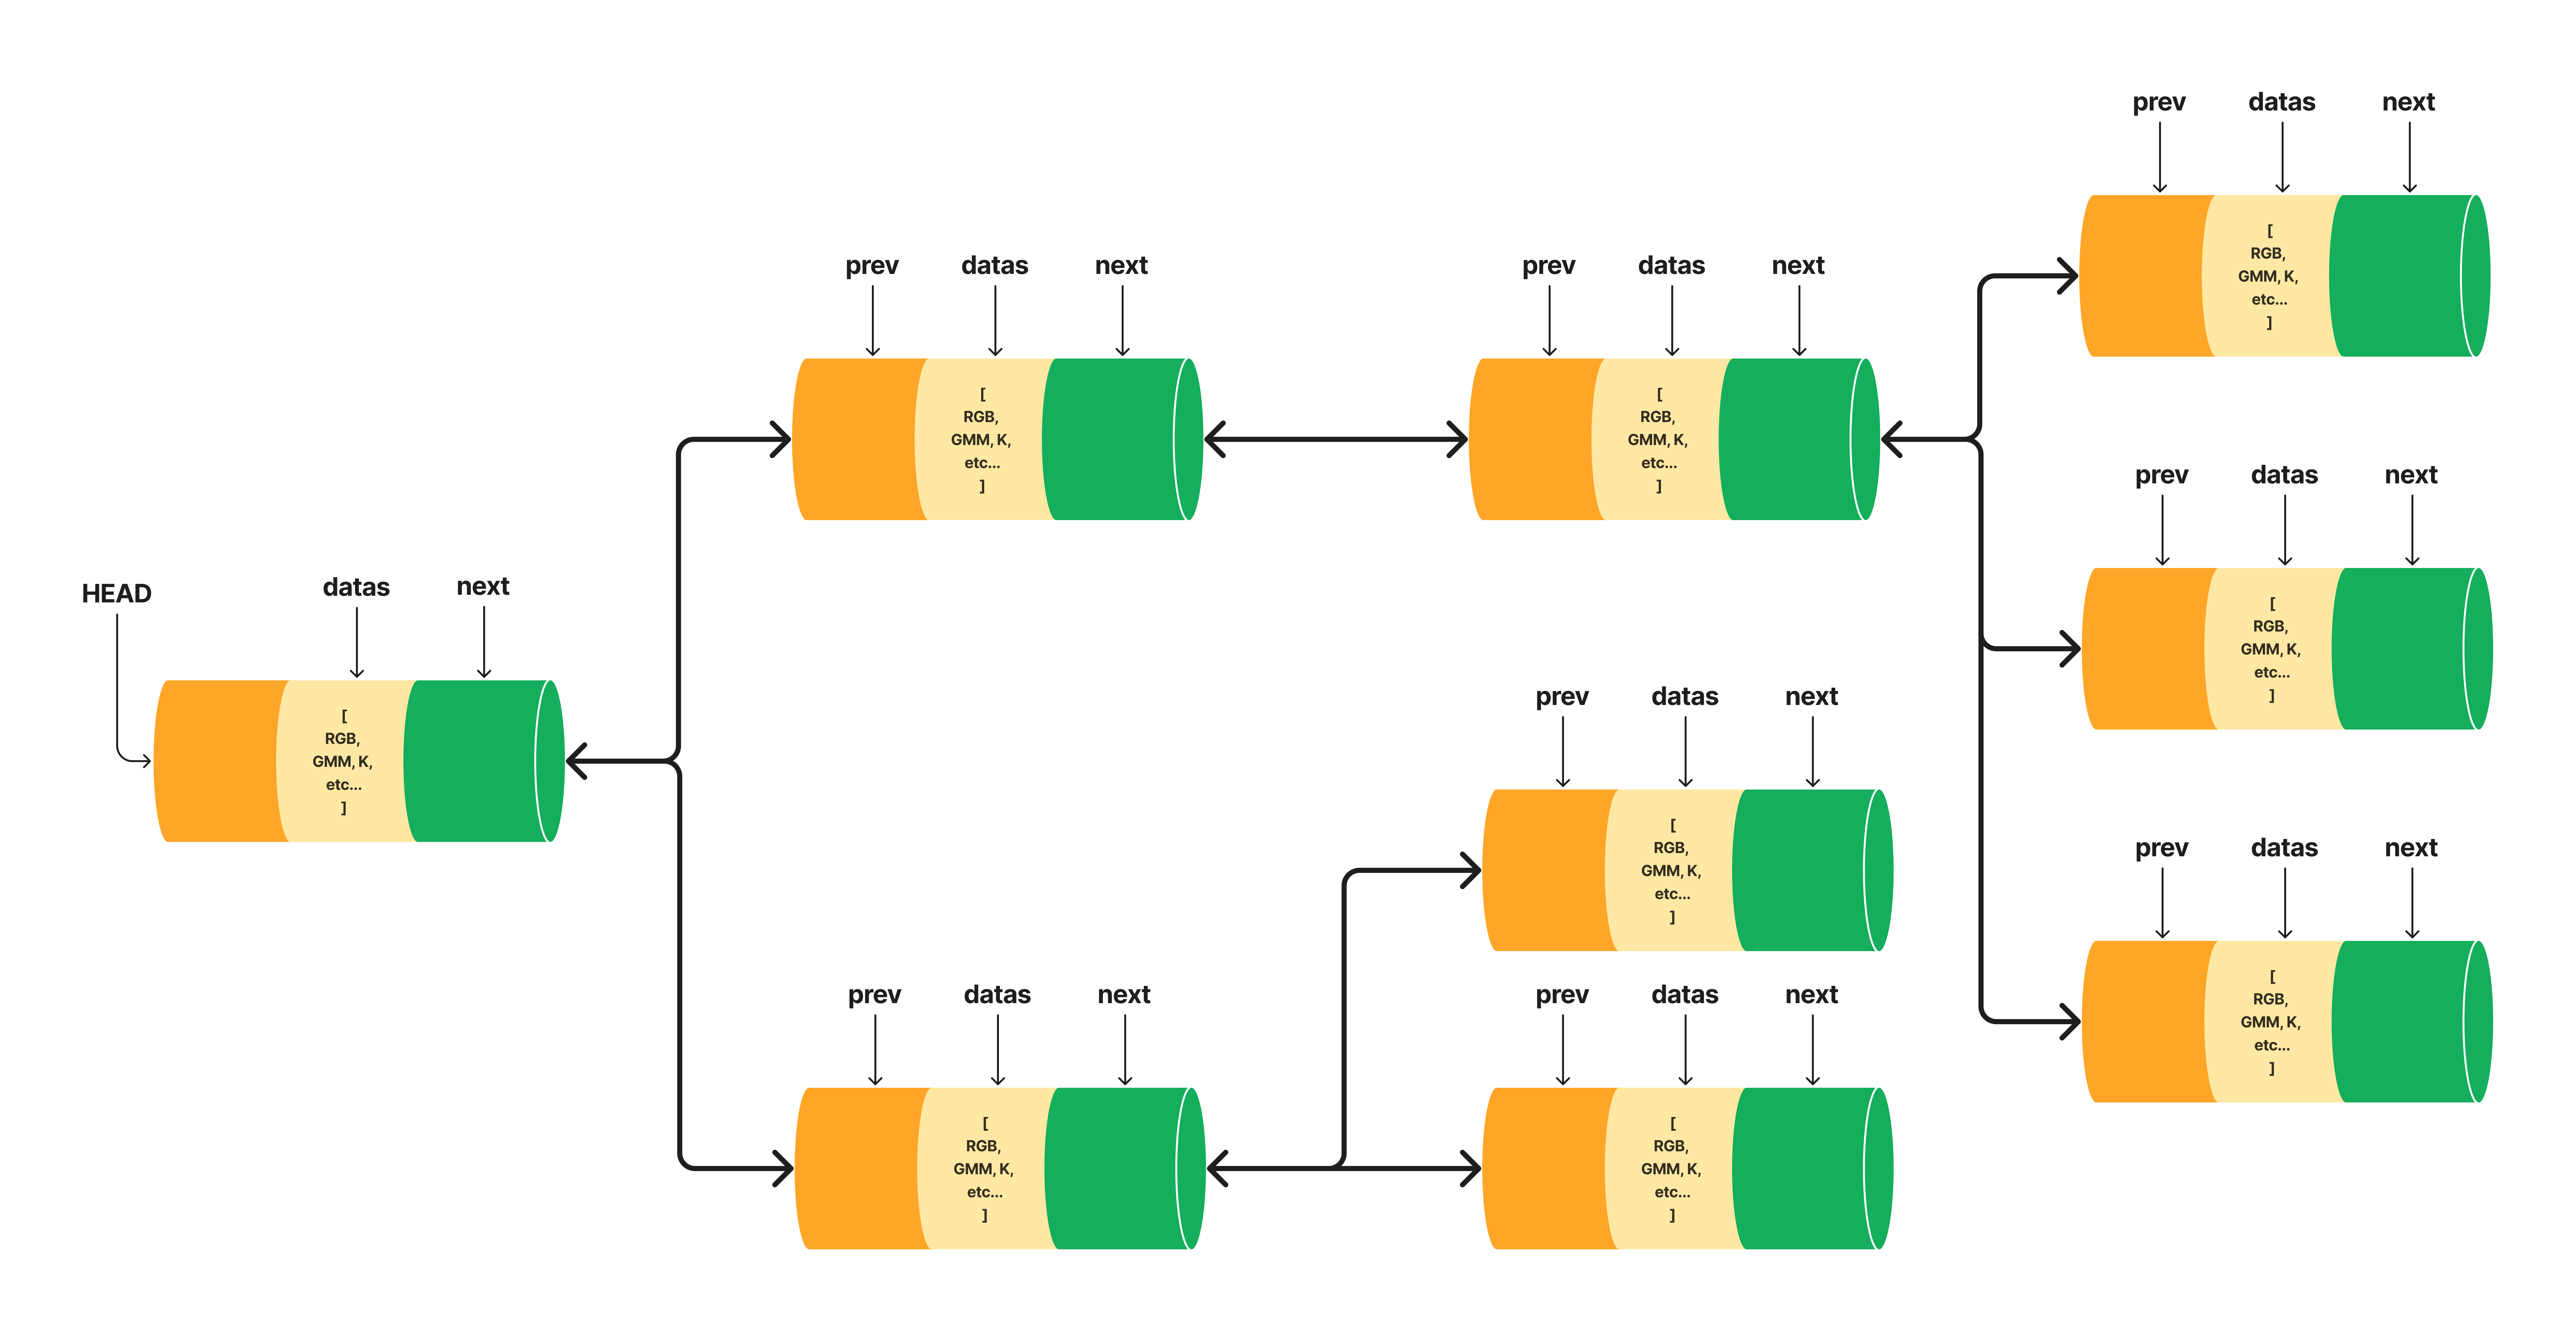
\includegraphics[width=0.8\textwidth]{gambar/tree_example.png}
	\caption{Representasi struktur data \emph{tree}}
\end{figure}

sehingga struktur data yang terbentuk dari \emph{tree} adalah sebagai berikut: 

\begin{lstlisting} [language=C++, caption=Struktur data \emph{tree}]
class Node {
    public:
        bool isForeground;
        double foregroundProbability;
        double backgroundProbability;
        vector<GaussianComponent> gmmComponents;

        Node* parent;
        vector<Node*> children;

        Node(bool isForeground, 
                double foregroundProbability, 
                double backgroundProbability ) {

            this->isForeground = isForeground;

            this->foregroundProbability = 
			foregroundProbability;

            this->backgroundProbability = 
			backgroundProbability;

            this->parent = nullptr;
        }
}

class Tree {
    private:
        Node* root;
    public:
        Tree() {
            root = nullptr;
        }

        Node* createNode(
            bool isForeground, 
            double foregroundProbability, 
            double backgroundProbability) {

            Node* newNode = new Node(
                isForeground, 
                foregroundProbability, 
                backgroundProbability);
            return newNode;
        }

        void insertChild(Node* parent, Node* child) {
            if (parent == nullptr || child == nullptr)
                return;

            child->parent = parent;
            parent->children.push_back(child);
        }
};

\end{lstlisting}

% ''' kalau mau dilanjutkan hingga di print '''
% int main() {
%     Tree tree;

%     Node* root = tree.createNode(0);
%     Node* child1 = tree.createNode(1);
%     Node* child2 = tree.createNode(2);
%     Node* child3 = tree.createNode(3);
%     Node* child4 = tree.createNode(4);
%     Node* child5 = tree.createNode(5);
%     Node* child6 = tree.createNode(6);
%     Node* child7 = tree.createNode(7);  
%     Node* child8 = tree.createNode(8);  


%     tree.insertChild(root, child1);
%     tree.insertChild(root, child2);
%     tree.insertChild(child1, child3);
%     tree.insertChild(child2, child4);
%     tree.insertChild(child2, child5);
%     tree.insertChild(child3, child6);
%     tree.insertChild(child3, child7);
%     tree.insertChild(child3, child8);

%     return 0;
% }

\subsection{Graf}
Struktur data graf dipakai untuk merepresentasikan gambar citra luka, citra yang
di input akan berbentuk matriks dua dimensi yang mana terdiri dari baris, kolom, 
dan ranah warna RGB, graf selanjutnya dibangun dan menghubungkan antar \emph{node}
piksel, penulis membuat ilustrasi dari graf sebagai berikut 

\begin{figure}[H]
	\centering{}
	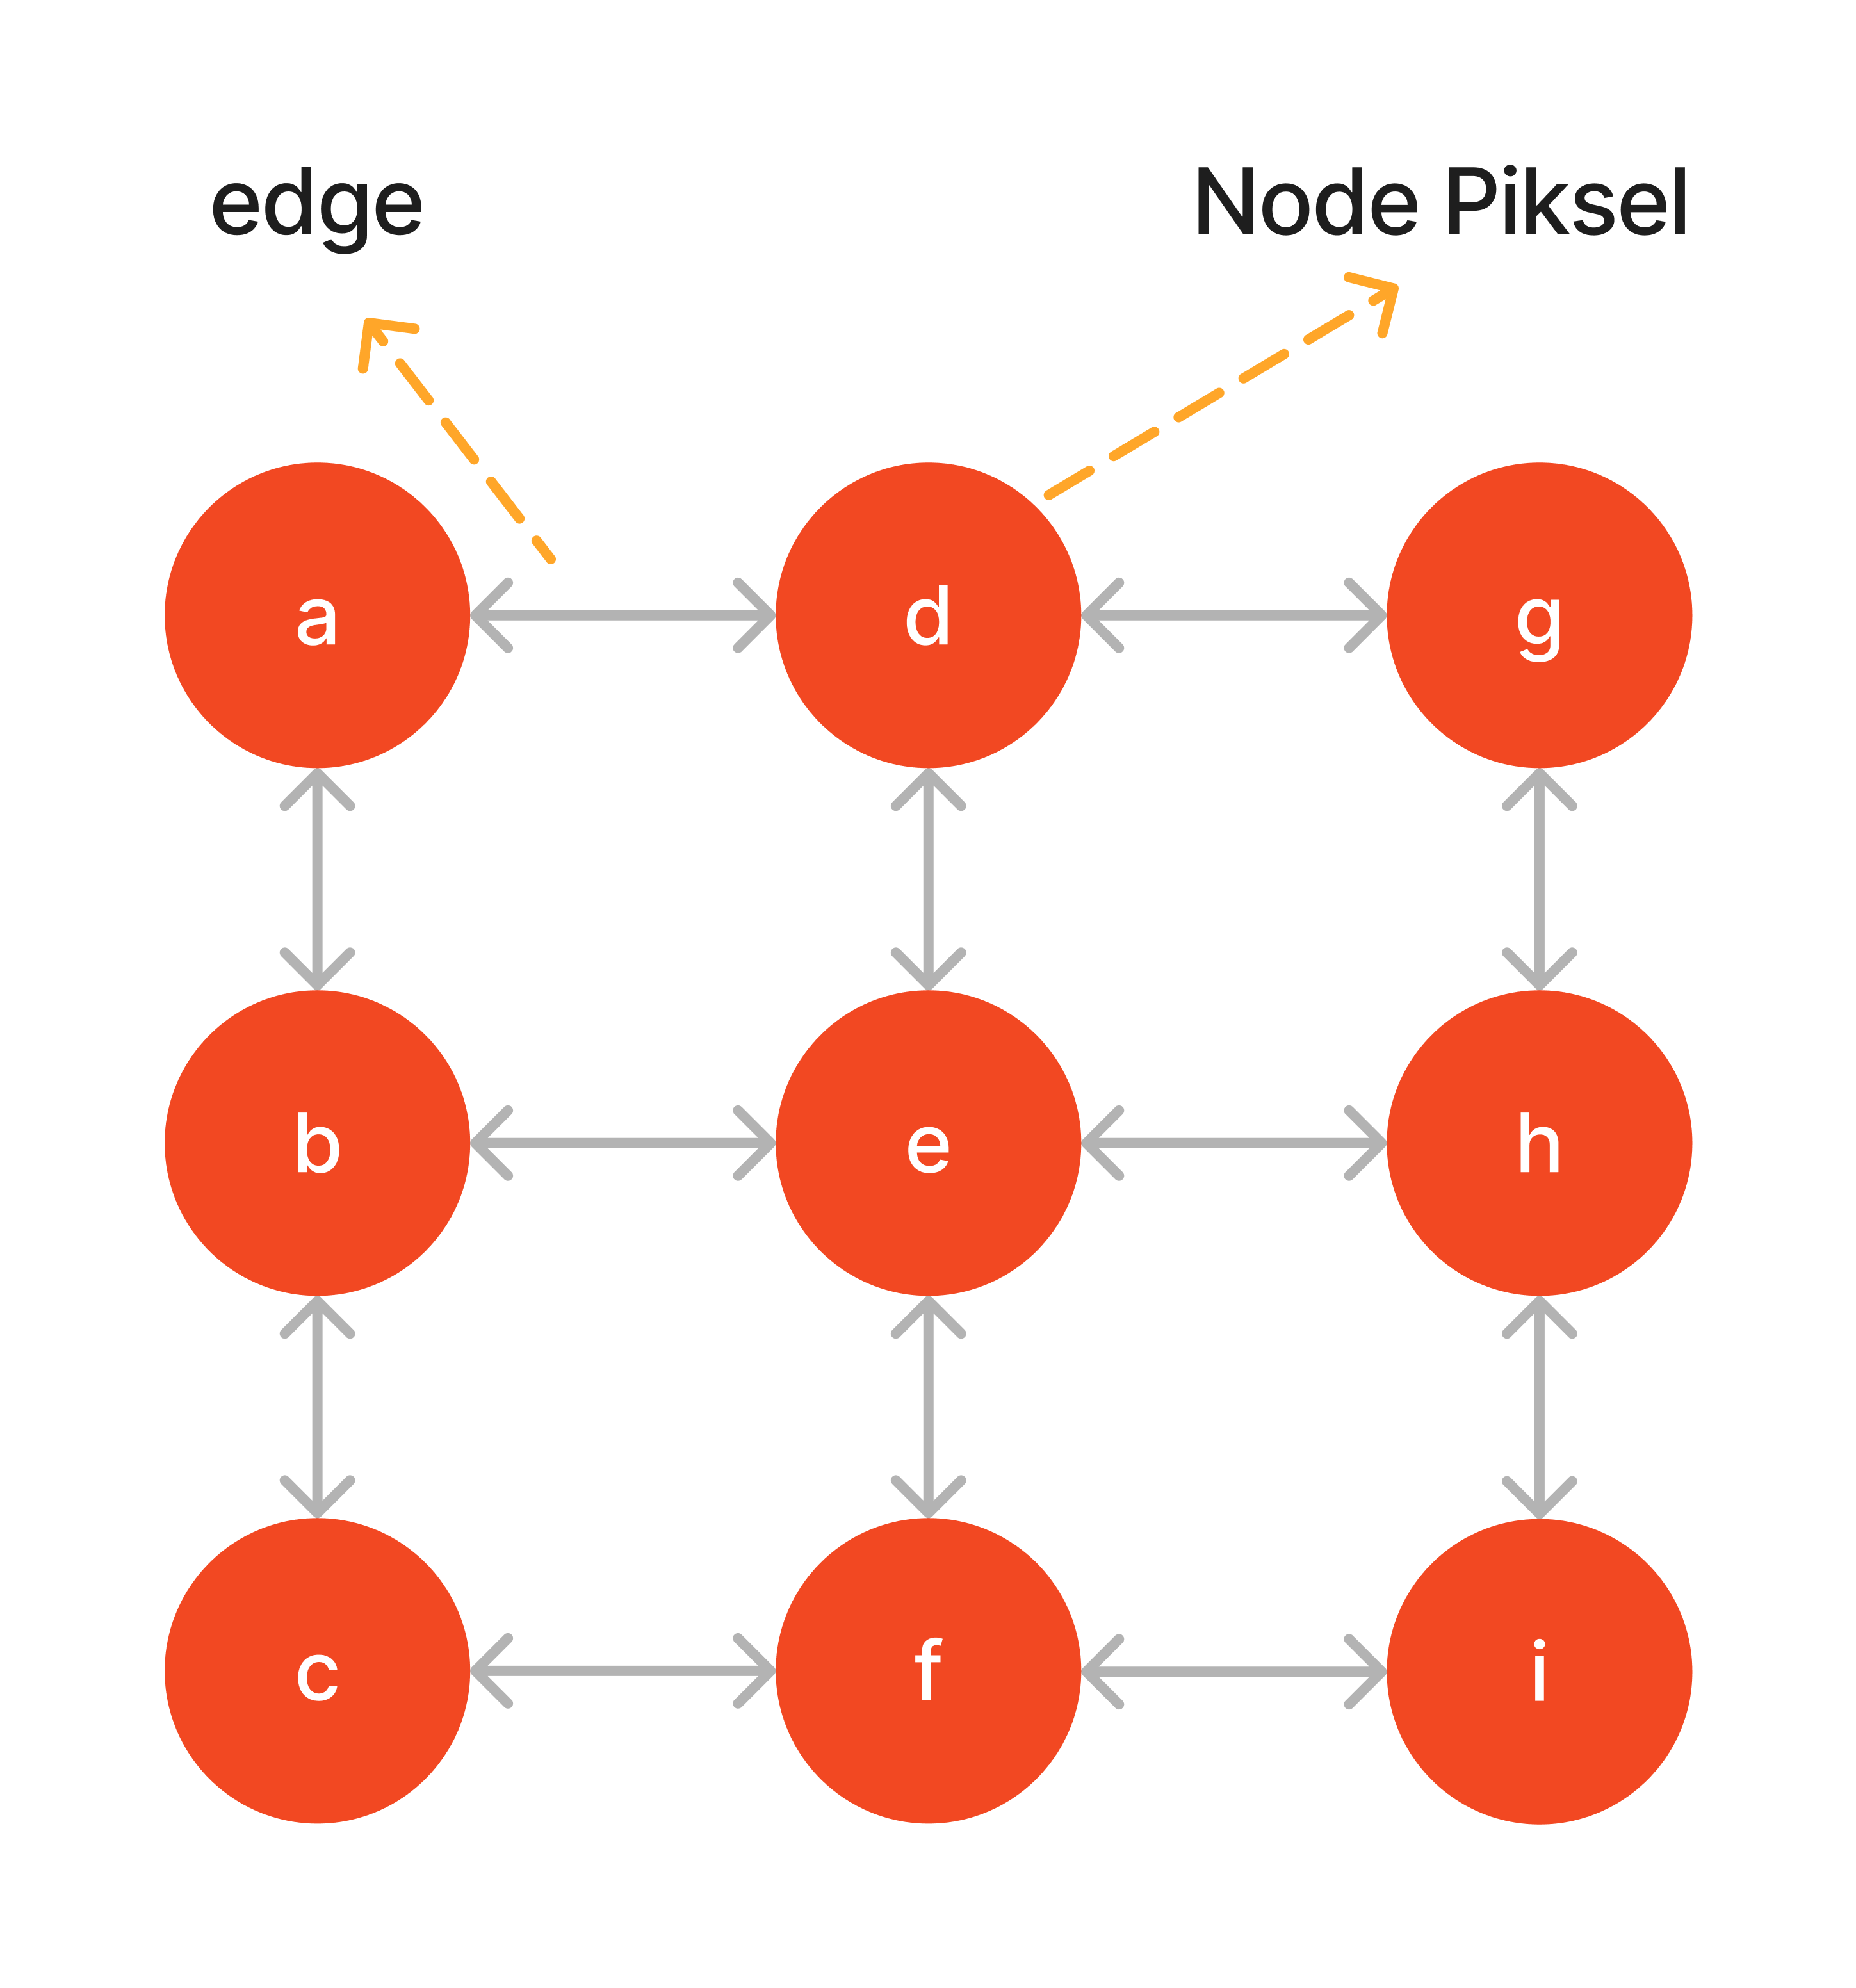
\includegraphics[width=0.3\textwidth]{gambar/graf.png}
	\caption{Ilustrasi graf terhadap piksel}
\end{figure}

Berikut struktur data untuk membangun graf
\begin{lstlisting} [language=C++, caption=Struktur data untuk membangun graf]

class Graph {
public:
    int num_nodes;
    vector<vector<int>> adj_list;

    // Constructor to initialize the graph with num_nodes vertices
    Graph(int num_nodes) {
        this->num_nodes = num_nodes;
        adj_list.resize(num_nodes);
    }

    // Function to add an edge between two vertices
    void add_edge(int u, int v) {
        adj_list[u].push_back(v);
        // adj_list[v].push_back(u); // If the graph is undirected
    }

    // Function to get edges of the graph
    vector<pair<int, int>> get_edges() {
        vector<pair<int, int>> edges;
        for (int u = 0; u < num_nodes; u++) {
            for (int v : adj_list[u]) {
                edges.push_back(make_pair(u, v));
            }
        }
        return edges;
    }
};
\end{lstlisting}
% int main() {
%     int num_nodes = 5; // Number of vertices in the graph
%     Graph graph(num_nodes);

%     // Adding edges to the graph
%     graph.add_edge(0, 1);
%     graph.add_edge(0, 4);
%     graph.add_edge(1, 2);
%     graph.add_edge(1, 3);
%     graph.add_edge(1, 4);
%     graph.add_edge(2, 3);
%     graph.add_edge(3, 4);

%     // Getting and printing the edges of the graph
%     vector<pair<int, int>> edges = graph.get_edges();
%     for (const auto& edge : edges) {
%         cout << edge.first << " -> " << edge.second << endl;
%     }

%     return 0;
% }

Setelah graf terbentuk, algoritma akan mulai mencari \emph{path} dari setiap \emph{node}
dengan ditentukannya dua \emph{node} khusus yaitu s (\emph{source}) dan t (\emph{sink}), 
dimana \emph{node} s akan menjadi  menjadi \emph{foreground} dan t menjadi \emph{background}.
Fungsi \emph{path} akan penulis jelaskan pada bagian \ref{section:skenario_eksperimen}.

\begin{figure}[H]
	\centering{}
	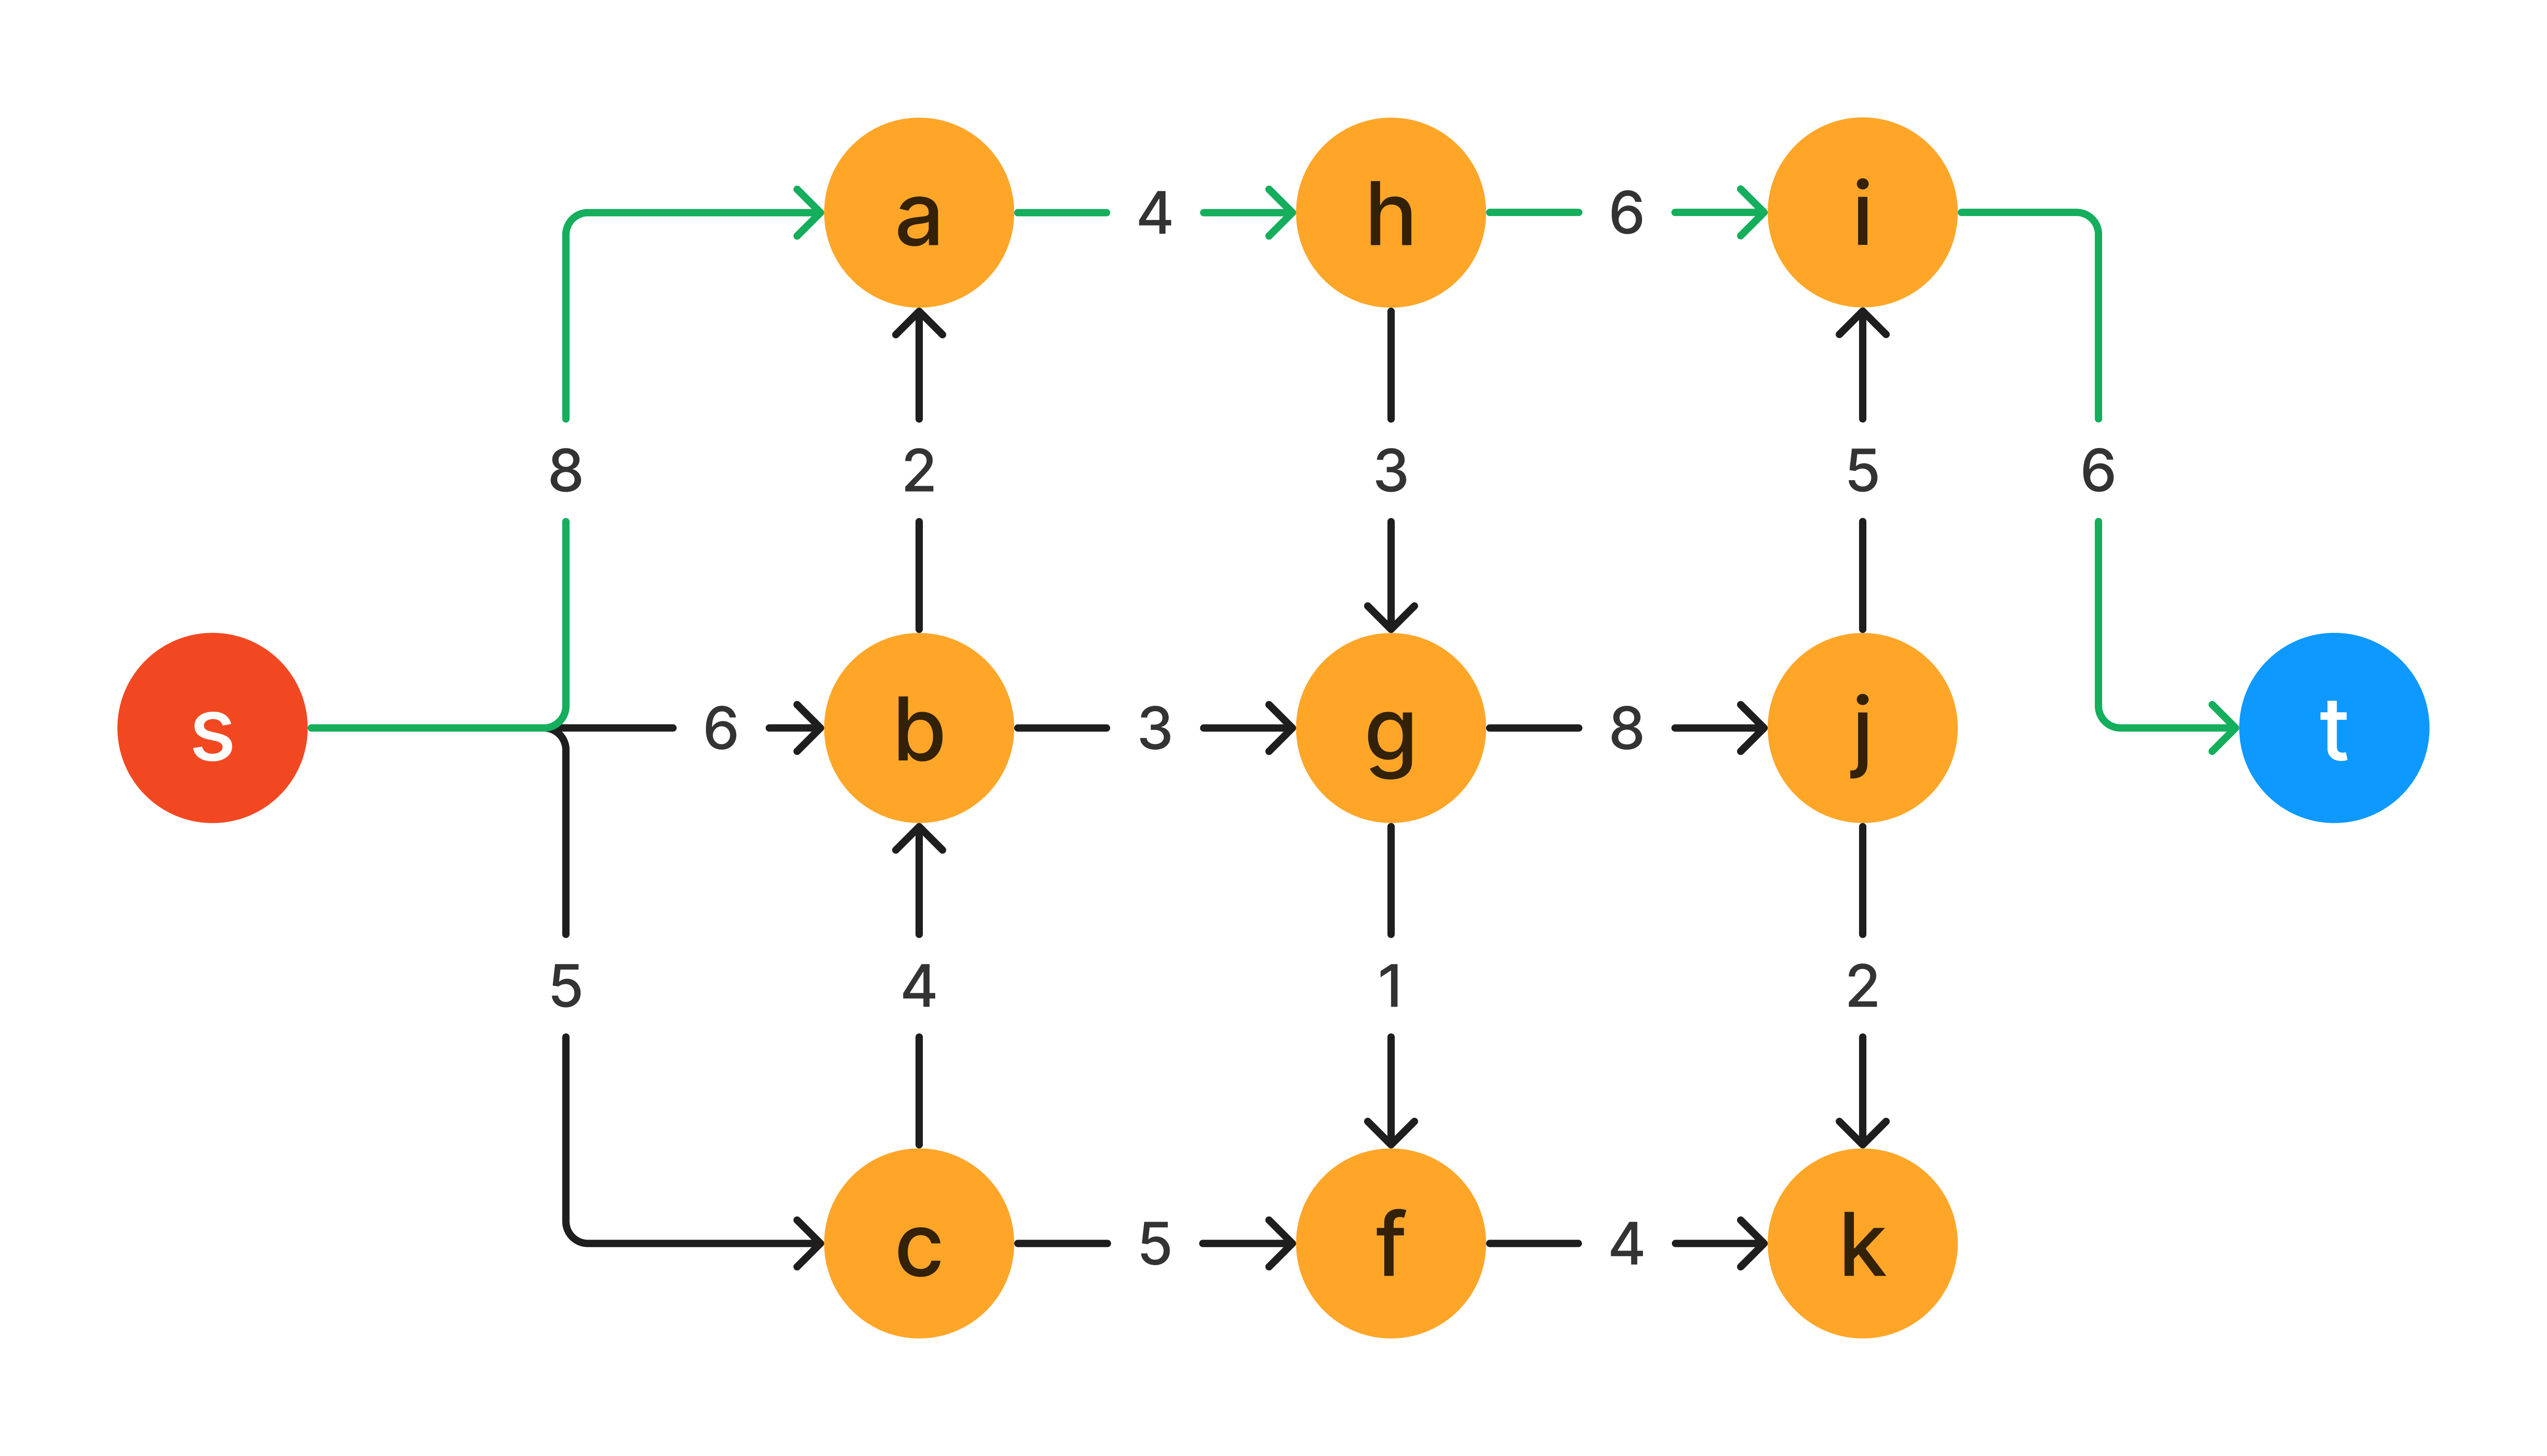
\includegraphics[width=0.6\textwidth]{gambar/contoh_path.png}
	\caption{Garis berwarna hijau menunjukkan \emph{path} s-a-h-i-t}
\end{figure}

Berikut struktur data untuk mencari \emph{path}
\begin{lstlisting} [language=C++, caption=Struktur data untuk mencari \emph{path}]

class Node {
    public:
        char name;
        int data;
        int capacity; // Capacity of the edge between this node and its parent
        Node* parent;
        vector<Node*> children;
        map<Node*, int> edges; // Map to store child nodes and their capacities


        Node(char name) {
            this->name = name;
            parent = nullptr;
            // capacity = 0; // Initialize capacity to 0
        }
    };

class Tree {
    private:
        Node* root;
    public:
    Tree() {
        root = nullptr;
    }

    void insertChild(Node* current, Node* next, int capacity) {
        Node* rootOfCurrent = getRoot(current);
        Node* rootOfNext = getRoot(next);

        if(next->parent == nullptr || rootOfNext->name == rootOfCurrent->name){

            next->parent = current;
            current->edges[next] = capacity;
            current->children.push_back(next);

            // get root of each node
            Node* nextRoot = getRoot(next);        
            cout << "node " << next->name 
            << " masuk ke tree " 
            << nextRoot->name ;
            cout << endl;

        }else if (rootOfNext->name != rootOfCurrent->name){
            cout << endl << "ada path di: "
            << next->name << endl;
            cout << "path nya adalah: "<< endl; 
            getPath(current, next);
            cout << "masuk ke tahap augmentasi" 
            << endl << endl;
        }  
        
    }

    // Add this helper function to get the capacity between two nodes
    int getEdgeCapacity(Node* parent, Node* child) {
        // Find the edge connecting the parent and child nodes
        auto it = parent->edges.find(child);
        if (it != parent->edges.end()) {
            return it->second; // Return the capacity of the edge
        }
        return 0; // Return 0 if the edge is not found (should not happen if the tree is correctly constructed)
    }
    

    void display(Node* node, int depth = 0) {

        if (node == nullptr)
            return;

        // Print current node with indentation
        for (int i = 0; i < depth; ++i) {
            cout << "    ";
        }
        cout << "|-- " << node->name << " (Capacity: " << node->capacity << ")" << endl;

        // Recursively display children
        for (Node* child : node->children) {
            display(child, depth + 1);
        }
    }

    void displayTree(Node* root) {
        cout << endl << "Tree dari Search Node " 
        << root->name << " adalah: " << endl;
        display(root);
    }

    Node* getRoot(Node* child) {

        Node* current = child;
        while (current->parent != nullptr) {
            current = current->parent;
        }

        return current;
    }

    vector<Node*> getLeafNodes(Node* node) {
        vector<Node*> leafNodes;

        if (node == nullptr){
            return leafNodes;
        }

        if (node->children.empty()) {
            leafNodes.push_back(node);
        } else {
            for (Node* child : node->children) {
                vector<Node*> childLeafNodes = 
                getLeafNodes(child);

                leafNodes.insert(
                leafNodes.end(), 
                childLeafNodes.begin(), 
                childLeafNodes.end()
                );
            }
        }        
        return leafNodes;
    }

    void displayLeafNodes(Node* root) {
        vector<Node*> leafNodes = getLeafNodes(root);
        cout << "Leaf nodes: ";
        for (Node* leafNode : leafNodes) {
            cout << leafNode->name << " ";
        }
        cout << endl;
    }
    
    bool getPathToRoot(Node* leaf, 
    vector<char>& path) {
        if (leaf == nullptr)
            return false;

        Node* current = leaf;
        while (current != nullptr) {
            path.push_back(current->name);
            current = current->parent;
        }

        return true;
    }
    
    vector<char> getPathFromLeafToRoot(Node* leaf) {
        vector<char> path;
        getPathToRoot(leaf, path);
        return path;
    }

    void displayLeafToRoot ( Node* leaf) {
        vector<char> path = 
        getPathFromLeafToRoot(leaf);
        getPathToRoot(leaf, path);

        // Display the path
        if(path[path.size()-1] != 't'){
            reverse(path.begin(), path.end());
        }
        cout << "Path from leaf " << leaf->name 
        << " to root:" << endl;
        for (int i = 0; i < path.size(); i++) {
            cout << path[i];
            if(i != path.size() -1){
                cout<< "->";
            }
        }
        cout << endl;
    }

    void getPath(Node* current, Node* next){
        vector<char> tmp_current = 
        getPathFromLeafToRoot(current);
        vector<char> tmp_next = 
        getPathFromLeafToRoot(next);
        vector<char> path;
        int totalCapacity = 0;

        for (char cek : tmp_current){
            cout<< cek ;
        };

        cout<<endl;

        for (char cek2 : tmp_next){
            cout<< cek2;
        };

        cout<< endl;



        if(tmp_current[tmp_current.size() - 1] == 't'){

            reverse(tmp_next.begin(), tmp_next.end());

            for(char node : tmp_next){
                path.push_back(node);
                if (path.size() > 1) {
                    Node* parent = next->parent;
                    int capacity = getEdgeCapacity(parent, next);
                    totalCapacity += capacity;
                    cout << "Capacity from " << parent->name << " to " << next->name << ": " << capacity << endl;
                }
            }
            for(char node : tmp_current){
                path.push_back(node);
                if (path.size() > 1) {
                    Node* parent = current->parent;
                    int capacity = getEdgeCapacity(parent, current);
                    totalCapacity += capacity;
                    cout << "Capacity from " << parent->name << " to " << next->name << ": " << capacity << endl;
                }
            }
        }else{
            
            reverse(tmp_current.begin(), tmp_current.end());

            for(char node : tmp_current){
                path.push_back(node);
                if (path.size() > 1) {
                    Node* parent = current->parent;
                    int capacity = getEdgeCapacity(parent, current);
                    totalCapacity += capacity;
                    cout << "Capacity from cu " << parent->name << " to " << current->name << ": " << capacity << endl;
                }
            }
            for(char node : tmp_next){
                path.push_back(node);
                if (path.size() > 1 && next->parent != nullptr) {
                    Node* parent_tmp = next->parent;
                    // cout<< parent->name;
                    int capacity = getEdgeCapacity(parent_tmp, next);
                    totalCapacity += capacity;
                    cout << "Capacity from ci " << parent_tmp->name << " to " << next->name << ": " << capacity << endl;
                    next = parent_tmp;
                }
            }
        }
        for (char i : path) {
            cout << i;
        }
    }
};
\end{lstlisting}
% int main() {
% 	// Create Tree S and T
% 	Tree tree_S;
% 	Tree tree_T;
% 	// Create root node s and t
% 	Node* root_S = new Node('s');
% 	Node* root_T = new Node('t');

% 	Node* nodeA = new Node('a');
% 	Node* nodeB = new Node('b');
% 	Node* nodeC = new Node('c');
% 	Node* nodeH = new Node('h');
% 	Node* nodeG = new Node('g');
% 	Node* nodeF = new Node('f');
% 	Node* nodeI = new Node('i');
% 	Node* nodeJ = new Node('j');

% 	tree_S.insertChild(root_S, nodeA);
% 	tree_S.insertChild(root_S, nodeB);
% 	tree_S.insertChild(root_S, nodeC);
% 	tree_T.insertChild(root_T, nodeI);
% 	tree_S.insertChild(nodeA, nodeH);
% 	tree_S.insertChild(nodeB, nodeG);
% 	tree_S.insertChild(nodeC, nodeF);
% 	tree_T.insertChild(nodeI, nodeH);
% 	tree_T.insertChild(nodeI, nodeJ);
%    return 0;
% }

\subsection{Algoritma \emph{GrabCut}}
Struktur data penelitian algoritma \emph{GrabCut} pada penelitian kali ini sebagai 
sebagai berikut: 

\begin{lstlisting} [language=C++, caption=Struktur data GrabCut]
// Struktur Data GrabCut
#include <iostream>
#include <opencv2/core/core.hpp>
#include <opencv2/highgui/highgui.hpp>
#include <boost/numeric/ublas/matrix.hpp>
#include <boost/numeric/ublas/vector.hpp>
#include <vector>
#include <algorithm>
#include <numeric>
#include <cmath>
#include <map>

class GrabCut {
private:
    cv::Mat gambar;
    int rows, cols;
    cv::Mat gambar_mask;
    int komponen_gmm;
    int nilai_gamma;
    int nilai_beta;

public:
    GrabCut(const cv::Mat& gambar, const cv::Mat& gambar_mask, int rect[4] = nullptr, int komponen_gmm = 5) {
        this->gambar = gambar;
        this->rows = gambar.rows;
        this->cols = gambar.cols;
        this->gambar_mask = gambar_mask;
        this->komponen_gmm = komponen_gmm;
        this->nilai_gamma = 50;
        this->nilai_beta = 0;
    }

    void inisiasi_piksel(){}

    void init_assign_gmm(){}

    void memperbarui_gmm(){}

    void hitung_smoothness(){}

    void bangun_graf(){}

    void graphcut_segmentation(){}
};

class GaussianMixture {
private:
    int komponen_gmm;
    int jumlah_fitur;
    vector<int> jumlah_sampel;
    ublas::vector<double> coefs;
    ublas::matrix<double> means;
    ublas::matrix<double> covariances;

public:
    GaussianMixture(const ublas::matrix<double>& X, int komponen_gmm = 5) {
        this->komponen_gmm = komponen_gmm;
        this->jumlah_fitur = x[1].size();
        this->jumlah_sampel = ublas::zero_vector<double>(komponen_gmm);

        this->coefs = ublas::zero_vector<double>(komponen_gmm);
        this->means = ublas::zero_matrix<double>(komponen_gmm, jumlah_fitur);
        this->covariances = ublas::zero_matrix<double>(komponen_gmm, jumlah_fitur * jumlah_fitur);
    }

    void init_rand(){}

    void dis_mult(){}

    void prob_calc(){}

    void learn_gmm(){}

    void count_params(){}

}

class GraphCut {
public:

    void build_graph(){}

    void run(){}

    void growth(){}

    void augmentation(){}

    void adoption(){}
}
\end{lstlisting}

\section{Algoritma Segmentasi Gambar dengan Metode \emph{GrabCut}}

Algoritma \emph{GrabCut} terdiri dari gabungan beberapa algoritma lain, yaitu 
pemrosesan oleh algoritma GMM dan minimisasi energi oleh algoritma \emph{GraphCut},
berikut algoritma dari \emph{GrabCut}:  

\begin{algorithm}                     
\caption{Algoritma segmentasi gambar dengan \emph{GrabCut} (\cite{Rother:2004})}          
\label{algo:grabcut}                          
\begin{algorithmic}                    % enter the algorithmic environment
    % \State $\textbf{From \xspace} GaussianMixtureModels \textbf{\xspace Import \xspace} GaussianMixture$
    \State $gambar \gets \Call{loadImage}$  \Comment{Input gambar 2.jpg}
    \State $\textbf{bool } kotak \gets false$ \Comment{Inisiasi keberadaan kotak}
    \State $\textbf{bool } drawing \gets false$ \Comment{Inisiasi keberadaan brush}
    \State $iy, ix \gets int$
    \State $gambar2 \gets \Call{Copy}{gambar}$
    \State $mask \gets \Call{ublas::zero\textunderscore matrix<double>}{gambar.shape[0], gambar.shape[1]}$
    \State $map<string, string> flagsColor$
    \State $map<string, integer> flagsValue$
    
    \State $flagsColor['bg'], flagsColor['fg']  \gets 'black', 'white'$
    \State $flagsValue['bg'], flagsValue['fg'], flagsValue['prob\textunderscore bg'], flagsValue['prob\textunderscore fg'] \newline
     \gets 0, 1, 2, 3$
    
    \\
    % GrabCut Class
    \State $komponen\textunderscore piksel \gets \newline
    \hspace*{2em} \Call{ublas::zero\textunderscore matrix<double>}{gambar.shape[0], gambar.shape[1]}$
    \State $\textbf{array } kotak\textunderscore lok[4] \gets [...]$
    % \State $flagsValue['bg'] \gets 0$
    % \State $flagsValue['prob\textunderscore bg'] \gets 2$
    % \State $flagsValue['prob\textunderscore fg'] \gets 3$

    % \State $flags['bg'] \gets ['black', 0]$
    % \State $flags['fg'] \gets ['white', 1]$
    % \State $flags['pr\textunderscore bg'] \gets ['red', 2]$
    % \State $flags['pr\textunderscore fg'] \gets ['blue', 3]$
    \\
    \Function{MouseHandler}{$event, x, y, flagsColor, flagsValue, param$}
        \If{$event == \Call{cv}{EVENT\textunderscore RBUTTON}$} 
            \State $ix, iy = x, y$
            \State $\Call{cv.rectangle}{gambar, (ix, iy), (x, y), flagsColor['warna'], 2}$
            \State $kotak \gets True$
            \State $kotak\textunderscore lok[4] \gets [min(ix, x), min(iy, y), abs(ix-x), abs(iy-y)]$
        \EndIf 
        \If{$event == \Call{cv}{EVENT\textunderscore LBUTTON}$} 
            \State $drawing \gets True$
            \State $\Call{cv.circle}{gambar, (x, y), 3, flagsColor['warna'], -1}$
            \State $\Call{cv.circle}{mask, (x, y), 3, flagsValue['value'], -1}$
            \State $drawing \gets False$
        \EndIf 
    \EndFunction
    \\
\algstore{algo:algo_all}
\end{algorithmic}
\end{algorithm}

\begin{algorithm}                     
\begin{algorithmic}                    % lanjutan algo_all di atas
\algrestore{algo:algo_all}

    \\
    \Comment{\textbf{ (Algorithm \ref{algo:intialize}) } Inisiasi TU = 1 untuk piksel didalam kotak, gambar \ref{gambar:2.6} }

    \Function{inisasi\textunderscore piksel}{$mask$}
        \If{$kotak\textunderscore lok[4] \neq None $} 
            \State $mask[kotak\textunderscore lok[...]] = 1$ 
        \EndIf
        \State $idx\textunderscore bg \gets bg['value'] \textbf{ or } pr\textunderscore bg['value']$
        \State $idx\textunderscore fg \gets fg['value'] \textbf{ or } pr\textunderscore fg['value']$
    \EndFunction

    \\ 
    \Comment{\textbf{ (Algorithm \ref{algo:assign_GMM}) } Inisiasi dan \emph{Assign} GMM ke setiap piksel, tahap 1 gambar \ref{gambar:2.6} }
    \Function{init\textunderscore assign\textunderscore gmm}{$idx\textunderscore bg, idx\textunderscore fg$}
        \State $GMM\textunderscore FG \gets GaussianMixture(idx\textunderscore fg)$
        \State $GMM\textunderscore BG \gets GaussianMixture(idx\textunderscore bg)$
        \State $\Call{GMM\textunderscore FG.dis\textunderscore mult}{idx\textunderscore fg}$
        \State $\Call{GMM\textunderscore BG.dis\textunderscore mult}{idx\textunderscore bg}$
    \EndFunction

    \\ 
    \Comment{\textbf{ (Algorithm \ref{algo:learn_GMM}) } mempelajari parameter GMM, tahap 2 gambar \ref{gambar:2.6} }
    \Function{memperbarui\textunderscore gmm}{}
        \State $\Call{GMM\textunderscore FG.count\textunderscore params}{gambar[idx\textunderscore fg], komponen\textunderscore piksel[idx\textunderscore fg]}$
        \State $\Call{GMM\textunderscore BG.count\textunderscore params}{gambar[idx\textunderscore bg], komponen\textunderscore piksel[idx\textunderscore bg]}$
    \EndFunction

    \\ 
    \Comment{\textbf{ (Algorithm \ref{algo:mincut_algorithm}) } segmentasi piksel, tahap 3 gambar \ref{gambar:2.6} }
    \Function{gc\textunderscore segmentation}{}
        \State $\textbf{vector<int> } gc\textunderscore graph \gets \Call{build\textunderscore graph}{edges, n\textunderscore piksel}$
        \State $\Call{mincut\textunderscore segmentation}{gc\textunderscore graph, gc\textunderscore sink, gc\textunderscore source, gc\textunderscore graph\textunderscore capacity}$
    \EndFunction
\end{algorithmic}
\end{algorithm}

\begin{algorithm}                     
    \caption{Algoritma inisialisasi \emph{bounding box} pada area luka}          
    \label{algo:intialize}                          
    \begin{algorithmic}                    % enter the algorithmic environment
        \\  \Comment{Tahap inisialisasi pada gambar \ref{gambar:2.6}}
    
        \Function{inisasi\textunderscore piksel}{$mask$}

            \If {$kotak\textunderscore lok \neq None$}
                \State $mask[kotak\textunderscore lok[1]:kotak\textunderscore lok[1] + 
                kotak\textunderscore lok[3],\newline  
                \hspace*{4em} kotak\textunderscore lok[0]: kotak\textunderscore lok[0] + 
                kotak\textunderscore lok[2]] \gets flags['fg']['value']$
            \EndIf

            \State $idx\textunderscore bg \gets \textbf{where}(mask == flags['bg']['value']  \textbf{\xspace or\xspace}  \newline 
            \hspace*{4em} mask == flags['pr\textunderscore bg']['value'])$
            \State $idx\textunderscore fg \gets \textbf{where}(mask == flags['fg']['value']  \textbf{\xspace or\xspace}  \newline 
            \hspace*{4em} mask == flags[''pr\textunderscore fg']['value'])$
        
        \EndFunction
    % \algstore{algo:initialize}
    \end{algorithmic}
\end{algorithm}
        

\begin{algorithm}                     
    \caption{Algoritma inisiasi dan \emph{Assign} GMM pada setiap piksel citra}          
    \label{algo:assign_GMM}                          
    \begin{algorithmic}                    % enter the algorithmic environment

    \State $typedef ublas::matrix<double> Matrix;$
    \State $typedef ublas::vector<double> Vector;$

    \Function{init\textunderscore assign\textunderscore gmm}{$idx\textunderscore bg, idx\textunderscore fg$}
        \State $GMM\textunderscore BG \gets GaussianMixture(gambar[idx\textunderscore bg])$
        \State $GMM\textunderscore FG \gets GaussianMixture(gambar[idx\textunderscore fg])$

        \State $komponen\textunderscore piksel[idx\textunderscore bg] \gets \Call{GMM\textunderscore BG.dis\textunderscore mult}{gambar[idx\textunderscore bg]}$
        \State $komponen\textunderscore piksel[idx\textunderscore fg] \gets \Call{GMM\textunderscore FG.dis\textunderscore mult}{gambar[idx\textunderscore fg]}$
    \EndFunction
    \\
    \Function{dis\textunderscore mult}{$target$} \Comment{rumus \ref{eq:distribusi_multi}}
        \State $gauss\textunderscore score \gets  \Call{np.zeros}{target.shape[0]}$
        \State $\Call{init\textunderscore rand}{$target$}$
        \For{$k = 0; k < komponen\textunderscore gmm; k++$}
            \If{$coefs > 0$}
                \State $Vector XminMu \gets target - means[k]$
                \State $Vector trans\textunderscore XminMu \gets \Call{ublas::trans}{XminMu}$
                \State $Matrix inv\textunderscore cov = ublas::inv(self.covariances[ci])$
                \State $tmp\textunderscore dot \gets \Call{ublas::prod}{inv_cov, trans\textunderscore XminMu}$
                \State $tmp\textunderscore mult \gets \Call{ublas::element\textunderscore prod}{'ij,ij->i', \newline 
                \hspace*{6em} XminMu, ublas::trans(tmp\textunderscore dot)}$
                \State $pembagi \gets \Call{sqrt}{2* M.PI} * \Call{sqrt}{ublas::det(covarians[k])}$
                \State $gauss\textunderscore score \gets \frac{\Call{np.exp}{-0.5 * tmp\textunderscore mult}}{pembagi}$
            \EndIf
        \EndFor
        \State $\textbf{return } \Call{np.argmax}{gauss\textunderscore score}$
    \EndFunction
    \\
    \Function{init\textunderscore rand}{$target$}
        \State $\textbf{vector<int> } labelPix[target.shape[0]]$
        \For{$\textbf{int } i = 0; i < target.shape[0]; i++$}
            \State $labelPix[i] \gets rand() \mod 5;$
        \EndFor
        \State $\Call{count\textunderscore params}{target, labelPix}$
    \EndFunction
    \end{algorithmic}
\end{algorithm}

\begin{algorithm}
    \caption{Algoritma mempelajari parameter GMM}          
    \label{algo:learn_GMM}                 
    \begin{algorithmic}            % enter the algorithmic environment
        \\  \Comment{Tahap mempelajari GMM \ref{gambar:2.6}}
        \State $vector<int> unique\textunderscore labels;$
        \State $vector<int> labelCounts;$
    
        \Function{memperbarui\textunderscore GMM}{}
            \State $\Call{count\textunderscore params}{gambar[idx\textunderscore bg], komponen\textunderscore piksel[idx\textunderscore bg]} $
            \State $\Call{count\textunderscore params}{gambar[idx\textunderscore fg], komponen\textunderscore piksel[idx\textunderscore fg]} $
        \EndFunction

        \Function{count\textunderscore params}{$ublas::matrix<double> target,\newline 
        \hspace*{4em} ublas::matrix<double> labels$}
            \State $tie(unique\textunderscore labels, labelCounts) = uniqueWithCounts(labels);$

            \For{\textbf{int }k = 0; k < unique\textunderscore labels; k++}
                % \State $\textbf{int }n\textunderscore k\textunderscore idx \gets labelCounts[k]$
                \State $coefs[k] \gets labelCounts[k] / accumulate(labelCounts.begin(), labelCounts.end(), 0)$
                \State $means[k] \gets ublas::mean(target[k == labels])$
                \State $covariances[k] \gets ublas::trans(ublas::cov(target[k == labels]))$
            \EndFor
        \EndFunction

        \\ \Comment{Fungsi untuk mencari nilai unik k tiap piksel}
        \Function{$pair<vector<int>, vector<int>> \newline search\textunderscore uniques$}{$const ublas::matrix<double>\& labels$} 
            \State $vector<int> unique\textunderscore labels;$
            \State $vector<int> labelCounts;$
            \State $map<int, int> countMap;$
        
            \\ \Comment{Menghitung jumlah muncul nilai k}
            \For{const auto\& label : labels}
                \State $countMap[label]++;$
            \EndFor
        
            \\ \Comment{Memisahkan nilai unik dan jumlah kemunculannya}
            \For{const auto\& entry : countMap}
                \State $unique\textunderscore labels.push\textunderscore back(entry.first);$
                \State $labelCounts.push\textunderscore back(entry.second);$
            \EndFor
        
            \State $\textbf{return } make\textunderscore pair(unique\textunderscore labels, labelCounts);$
        \EndFunction
    \end{algorithmic}
\end{algorithm}

\begin{algorithm}
    \caption{Algoritma segmentasi oleh \emph{mincut}}          
    \label{algo:mincut_algorithm}                 
    \begin{algorithmic}            % enter the algorithmic environment
        \State $\textbf{vector<int> } edges$
        \State $\textbf{vector<double> } D\textunderscore score$
        \State $\textbf{vector<int> } gc\textunderscore graph\textunderscore capacity$
        \State $\textbf{int } n\textunderscore piksel \gets gambar.shape[0] * gambar.shape[1]$
        \State $\textbf{int } gc\textunderscore source \gets n\textunderscore piksel$
        \State $\textbf{int } gc\textunderscore sink \gets gc\textunderscore source + 1$

        \Function{$gc\textunderscore segmentation$}{$\textbf{vector<int> } edges, \textbf{int } n\textunderscore piksel$}  
            \State $\textbf{vector<int> } gc\textunderscore graph \gets \Call{build\textunderscore graph}{edges, n\textunderscore piksel}$
            \State $\Call{mincut\textunderscore segmentation}{gc\textunderscore graph, gc\textunderscore sink, gc\textunderscore source, gc\textunderscore graph\textunderscore capacity}$
        \EndFunction
    \end{algorithmic}
\end{algorithm}

\begin{algorithm}
    \caption{Membangun graf}          
    \label{algo:build_graph}                 
    \begin{algorithmic}            % enter the algorithmic environment
        \\  \Comment{Tahap membangun graf }

        \State $\textbf{vector<int> } idx\textunderscore bg \gets np.where(mask.reshape(-1) == flagsValue['bg'])$
        \State $\textbf{vector<int> } idx\textunderscore fg \gets np.where(mask.reshape(-1) == flagsValue['fg'])$
        \State $\textbf{vector<int> } idx\textunderscore pr \gets np.where(mask.reshape(-1) == flagsValue['prob\textunderscore bg'] 
        \textbf{ or } mask.reshape(-1) == flagsValue['prob\textunderscore fg'])$

        \Function{$build\textunderscore graph$}{$\textbf{vector<int> } edges, \textbf{int } n\textunderscore piksel$}  
        \State $\textbf{Graph } graph\textunderscore gc((n\textunderscore piksel + 2))$
        % \\
        % \\ \Comment{Membangun graf untuk \emph{t-links}}
            \For{\textbf{int } i in (idx\textunderscore bg[0], idx\textunderscore fg[0], idx\textunderscore pr[0])}
                \State $\Call{graph\textunderscore gc.add\textunderscore edge}{gc\textunderscore source, i}$
                \State $\Call{graph\textunderscore gc.add\textunderscore edge}{gc\textunderscore sink, i}$
                \State $D\textunderscore score = -np.log(GMM\textunderscore BG \textbf{ or } GMM\textunderscore FG \newline
                \hspace*{8em} .count\textunderscore prob(gambar.reshape(-1, 3)[idx\textunderscore pr]))$
            \EndFor
            \State $\Call{gc\textunderscore graph\textunderscore capacity.push\textunderscore back}{(D\textunderscore score)} $
        \EndFunction
    \end{algorithmic}
\end{algorithm}

\begin{algorithm}
    \caption{Menghitung nilai D pada rumus \ref{eq:rumus_energi2}}          
    \label{algo:count_prob}                 
    \begin{algorithmic}            % enter the algorithmic environment
        \State $\textbf{vector<double> } prob$
        \Function{$count\textunderscore prob$}{$\textbf{vector<int> } target$}  
            \State $prob \gets [\Call{dis\textunderscore mult}{target}]$
            \State $\textbf{return } ublas::dot(coefs, prob)$
        \EndFunction
    \end{algorithmic}
\end{algorithm}

\begin{algorithm}
    \caption{Segmentasi oleh algoritma \emph{mincut} \ref{gambar:2.6}}          
    \label{algo:mincut_segmentation}                 
    \begin{algorithmic}            % enter the algorithmic environment
        \\ \Comment{Inisialiasi A, Path, dan O}
        \State $\textbf{vector<Node*> }  active\textunderscore nodes$
        \State $\textbf{vector<Node*> }  orphans\textunderscore nodes$
        \State $\textbf{vector<Node*> }  paths \gets null$
        \State $\textbf{vector<double> } tree\textunderscore cap$


        \\ \Comment{Inisialiasi S dan T}
        \State $\textbf{Tree }  tree\textunderscore S$
        \State $\textbf{Tree }  tree\textunderscore T$
        \State $\textbf{Tree }  tree$
        

        \State $\textbf{Node*} root\textunderscore S \gets \textbf{new} Node(gc\textunderscore source)$
        \State $\textbf{Node*} root\textunderscore T \gets \textbf{new} Node(gc\textunderscore sink)$
        \State $active\textunderscore nodes \gets \Call{active\textunderscore nodes.push\textunderscore back}{gc\textunderscore source, gc\textunderscore sink}$
        % \State $$

        \Function{$mincut\textunderscore segmentataion$}{$\textbf{vector<int> } gc\textunderscore graph, gc\textunderscore sink, gc\textunderscore source, gc\textunderscore graph\textunderscore capacity$}  
            \While{$true$}
                \State $\Call{growth\textunderscore step()}{}$
                \If{$paths \neq 0$}
                    \State $\Call{augmentation\textunderscore step(gc\textunderscore sink, gc\textunderscore source)}{}$
                \EndIf
                \State $\Call{adoption\textunderscore step(gc\textunderscore sink, gc\textunderscore source)}{}$

                % \For{$...$}
                %     \State $...$
                % \EndFor
            \EndWhile
        \EndFunction
    \end{algorithmic}
\end{algorithm}

\begin{algorithm}
    \caption{tahap growth pada \emph{mincut} di bagian \ref{fase_growth}}          
    \label{algo:fase_growth}                 
    \begin{algorithmic}            % enter the algorithmic environment
        \Function{$growth\textunderscore step$}{}
            \State $\textbf{vector<Node*> } list\textunderscore neighbors $
            \State $\Call{search\textunderscore neighbors}{active\textunderscore nodes, tree\textunderscore cap}$
            \While{$active\textunderscore nodes \neq 0$}
                \For{$\textbf{int }i; i < list\textunderscore neighbors.size(); i++$}
                    \If{$tree\textunderscore cap[i] > 0$}
                        \If{$\textbf{tree.getRoot}(list\textunderscore neighbors[i]) == null$}
                            \State $tree.insertChild(active\textunderscore nodes[0], list\textunderscore neighbors[i])$
                        \ElsIf{$\textbf{tree.getRoot}(list\textunderscore neighbors[i]) \neq null \textbf{ and } \newline
                                \textbf{tree.getRoot}(list\textunderscore neighbors[i]) \neq \textbf{tree.getRoot}(active\textunderscore nodes[0])$}
                            \State $paths \gets tree.getPath(active\textunderscore nodes[0], list\textunderscore neighbors[i])$                    
                        \EndIf
                    \EndIf
                \EndFor
                \State $active\textunderscore nodes.pop()$
            \EndWhile
            \State $\textbf{return } paths \neq 0$
        \EndFunction
    \end{algorithmic}
\end{algorithm}

\begin{algorithm}
    \caption{tahap augmentasi pada \emph{mincut} di bagian \ref{fase_augmentation}}          
    \label{algo:fase_augmentation}                 
    \begin{algorithmic}            % enter the algorithmic environment
        \Function{$augmentation\textunderscore step$}{$\textbf{vector<int> } gc\textunderscore graph, gc\textunderscore sink, gc\textunderscore source$}
            \Call{$tree.get\textunderscore residu$}{paths, gc\textunderscore graph\textunderscore capacity}
            \For{$\textbf{int }i; i < path\textunderscore residu.size(); i++$}
                \If{$\textbf{tree.getRoot}(i[0]) == \textbf{tree.getRoot}(i[1]) == gc\textunderscore source$}
                    \State $\textbf{tree.setParentNull}(i[1])$
                    \State $orphans.push\textunderscore back(i[1])$
                \ElsIf{$\textbf{tree.getRoot}(i[0]) == \textbf{tree.getRoot}(i[1]) == gc\textunderscore sink$}
                    \State $\textbf{tree.setParentNull}(i[0])$
                    \State $orphans.push\textunderscore back(i[0])$
                \EndIf
            \EndFor
        \EndFunction
    \end{algorithmic}
\end{algorithm}

\begin{algorithm}
    \caption{tahap augmentasi pada \emph{mincut} di bagian \ref{fase_adoption}}          
    \label{algo:fase_adoption}                 
    \begin{algorithmic}            % enter the algorithmic environment
        \Function{$adoption\textunderscore step$}{$\textbf{vector<int> } gc\textunderscore graph, gc\textunderscore sink, gc\textunderscore source$}
            \State $\textbf{Node*} current\textunderscore orphans $
            \While{$orphans \neq 0$}
                \State $current\textunderscore orphans \gets orphans[0]$
                \State $\Call{search\textunderscore neighbors}{current\textunderscore orphans, tree\textunderscore cap}$
                \State $orphans.pop()$
                \For{$\textbf{int }i; i < list\textunderscore neighbors.size(); i++$}
                    \If{$tree.getRoot(list\textunderscore neighbors[i]) == \hfill \newline 
                    \hspace*{5em} tree.getRoot(current\textunderscore orphans)  \textbf{ and } \hfill \newline 
                    \hspace*{5em} tree.getEdgeCapacity(list\textunderscore neighbors[i],\newline 
                    \hspace*{5em} current\textunderscore orphans) > 0$} 
                        \State $tree.insertChild(list\textunderscore neighbors[i], current\textunderscore orphans)$     
                        \State $\textbf{break}$             
                    \EndIf 
                \EndFor
            \EndWhile
        \EndFunction
    \end{algorithmic}
\end{algorithm}


\pagebreak
\section{Alat dan Bahan Penelitian}
Pada penelitian kali ini, penulis menggunakan perangkat keras sebagai berikut:
\begin{enumerate}
    \item Laptop dengan prosesor AMD Ryzen 5 3500H \emph{series} dan \emph{RAM 16 GB}
    \item Koneksi berbasis Wi-Fi serta kuota internet dari ponsel pintar
    \end{enumerate}
Untuk perangkat lunak yang penulis gunakan sebagai berikut:
\begin{enumerate}
    \item Windows 11 64 bit OS
    \item Visual Studio Code sebagai \emph{Code Editor}
    \item Python 3 untuk menjalankan program Python
    \end{enumerate}

\section{Tahapan Penelitian} \label{section:tahapan_penelitian}
Dalam penelitian ini penulis melakukan perancangan penelitian terhadap citra luka 
yang akan di segmentasi antara objek luka dan latar belakang, perancangan yang akan
penulis lakukan yaitu 

\subsection{Persiapan \emph{dataset} input citra}

Sebelum melakukan inisiasi pada luka, penulis perlu menyiapkan \emph{dataset} luka, \emph{dataset}
ini kemudian penulis jadikan sampel data input citra. Sampel data dinilai baik 
ketika sampel tersebut mencerminkan populasi dari data tersebut (\cite{Rizki:2022}). 
Silva menggunakan 105 citra luka tentang segmentasi luka otomatis dengan menggunakan 
SVM dan Grabcut(\cite{Silva:2015}). Dalam penelitiannya Wang melakukan automasi segmentasi luka dengan
\emph{Deep Convolutional Neural Networks} menggunakan 2700 citra gambar luka (\cite{Wang:2015}).

Penulis menggunakan \emph{dataset} berjumlah 108, 37 data tidak dapat digunakan 
karena terdapat duplikasi dengan data lain sehingga tersedia 71 buah citra 
yang penulis jadikan sebagai populasi sekaligus sampel (sampel = populasi),
citra tersebut memiliki kategori sesuai dengan warna luka, yaitu luka hitam sebanyak
24 citra, luka kuning sebanyak 15 citra, dan luka merah 32 citra. \emph{Dataset}
penulis dapat dari penelitian luka Ns. Ratna Aryani, K.Kep, tahun 2018 (\cite{Aryani:2018})
yang terdapat pada repositori \url{https://github.com/mekas/InjuryDetection}.

Data awal yang penulis dapat adalah data-data yang berekstensi .xcf yang bisa 
dibuka menggunakan \emph{software} GIMP, pengolahan data sebelum deteksi menggunakan
\emph{GrabCut} dilakukan menggunakan \emph{software} Figma. Masing-masing \emph{dataset} 
didalamnya terdapat \emph{layer} citra (luka), \emph{layer} region (luka), dan 
\emph{path} sebagai berikut :

\begin{figure}[H]
	\centering
	  \begin{subfigure}{0.2\textwidth}
		\centering{}
		
\includegraphics[width=\textwidth]{gambar/gambar-3_2(a).png}
		\caption{}
	  \end{subfigure}%
	  \begin{subfigure}{0.2\textwidth}
		\centering{}
		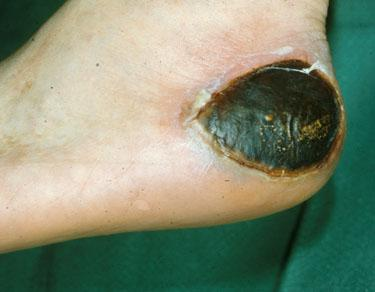
\includegraphics[width=\textwidth]{gambar/gambar-3_2(b).jpg}
		\caption{}
	  \end{subfigure}  
	  \begin{subfigure}{0.2\textwidth}
		\centering{}
		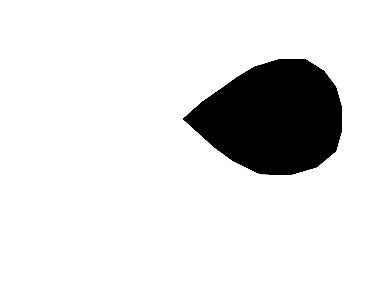
\includegraphics[width=\textwidth]{gambar/gambar-3_2(c).jpg}
		\caption{}
	  \end{subfigure}
	  \begin{subfigure}{0.2\textwidth}
		\centering{}
		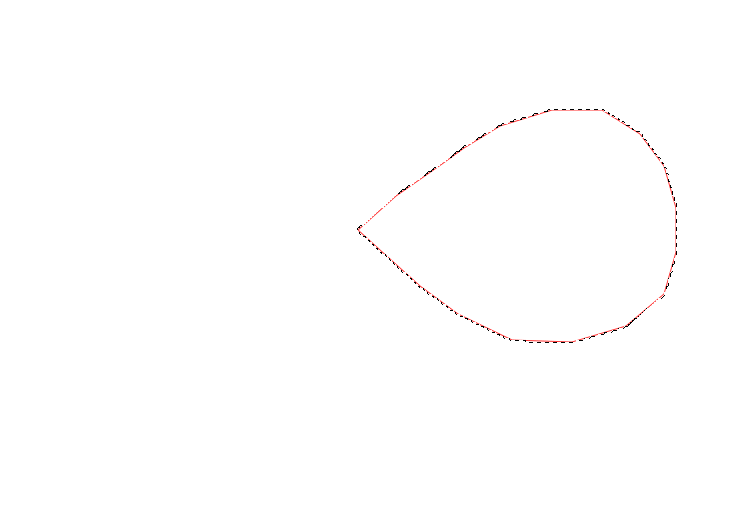
\includegraphics[width=\textwidth]{gambar/gambar-3_2(d).png}
		\caption{}
	  \end{subfigure}  
	\caption{
		(a)Data citra format .xcf, (b) \emph{layer} citra (luka), (c) \emph{layer} 
		region, (d)path
	 }
  \end{figure}

Langkah selanjutnya adalah penulis memasukkan data citra 2(b) ke dalam figma untuk
membuat \emph{layer} dan region (luka) dengan menggunakan \emph{pen tools}, hasil 
dari \emph{pen tools} akan berupa \emph{stroke} atau seperti path 2(d), kemudian 
penulis menduplikasi hasil path dan mengubahnya menjadi objek (\emph{fill object})
seperti 2(c).

\begin{figure}[H]
	\centering{}
	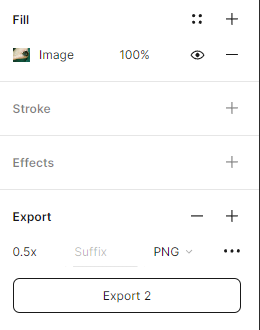
\includegraphics[width=0.3\textwidth]{gambar/gambar-3_4.png}
	\caption{Proses \emph{resize} citra gambar luka dengan ukuran 0.5 dari ukuran awal}
  \end{figure}

Setelah penulis melakukan \emph{resize} ukuran citra, selanjutnya penulis \emph{export}
\emph{layer} masing masing ke format .jpg.

% \begin{figure}[H]
% 	\centering{}
% 	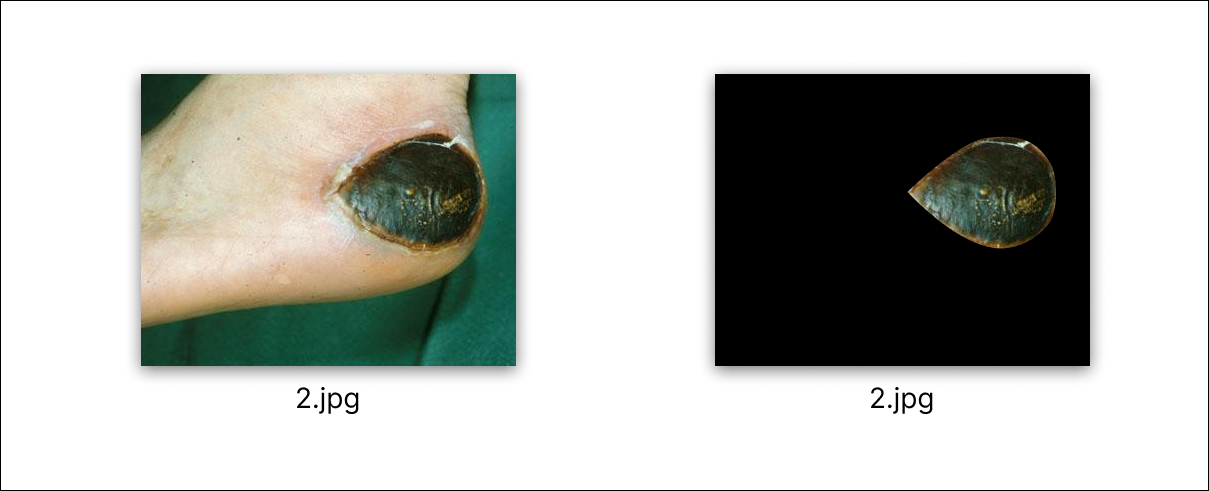
\includegraphics[width=\textwidth]{gambar/gambar-3_5.png}
% 	\caption{Citra gambar luka dan \emph{region} luka}
% \end{figure}

\subsection{Inisiai \emph{Bounding Box} di area luka}

Penulis memulai dengan menentukan kotak pembatas (\emph{bounding box}) yang mengelilingi 
objek yang ingin dipisahkan. Area di dalam \emph{bounding box} akan digunakan untuk membuat 
\emph{Trimap Unknown} \((T_{U})\), sementara area di luar \emph{bounding box} dianggap sebagai Trimap 
Background \((T_{B})\). Setiap piksel yang termasuk dalam \((T_{B})\) akan memiliki nilai 
\(\alpha_{n}\) sama dengan 0, sedangkan piksel yang termasuk dalam \((T_{U})\) akan memiliki nilai 
\(\alpha_{n}\) sama dengan 1. \emph{Bounding box} digunakan untuk mempercepat waktu komputasi algoritma dan meningkatkan 
akurasi segmentasi.

\begin{figure}[H]
	\centering{}
    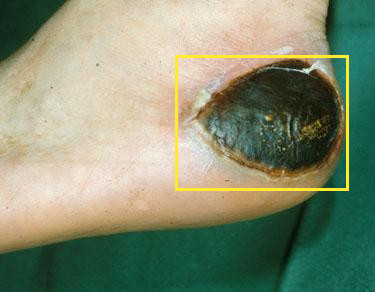
\includegraphics[width=0.3\textwidth]{gambar/rectangle.png}
	\caption{Inisiasi area objek luka dengan \emph{bounding box}}
\end{figure}

\subsection{Inisiasi GMM}

Pertama penulis akan melakukan inisiasi untuk tiap parameter GMM, di antaranya 
\(\{\mu, \Sigma \}\), pada algoritma \emph{grabcut} akan digunakan K = 5. Adapun
inisiasi yang dilakukan adalah membuat nilai random terhadap \(\mu\) dan \(\Sigma\).
setelah itu penulis menentukan \(\omega_k = \frac{1}{5}\), untuk \(k \in \{1, ..., 5\}\).
Distribusi gaussian yang akan digunakan untuk citra gambar berwarna yaitu distribusi 
gaussian \emph{multivariate} 2 dimensi atau 3 dimensi, sebagai ilustrasi gausian berdistribusi 
normal 2 dimensi dengan objek citra gambar luka berwarna :

% \begin{figure}[H]
% 	\centering
% 	\begin{subfigure}{0.3\textwidth}
% 		\centering{}
% 		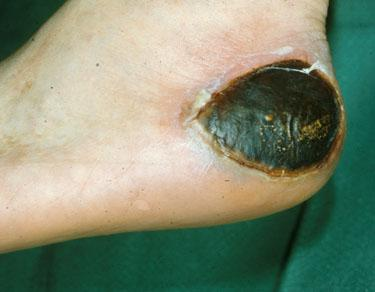
\includegraphics[width=\textwidth]{gambar/gambar-3_2(b).jpg}
% 		\caption{}
% 	\end{subfigure}
%     % \hfill% or \hspace{5mm} or \hspace{0.3\textwidth}
% 	\begin{subfigure}{0.3\textwidth}
% 		\centering{}
% 		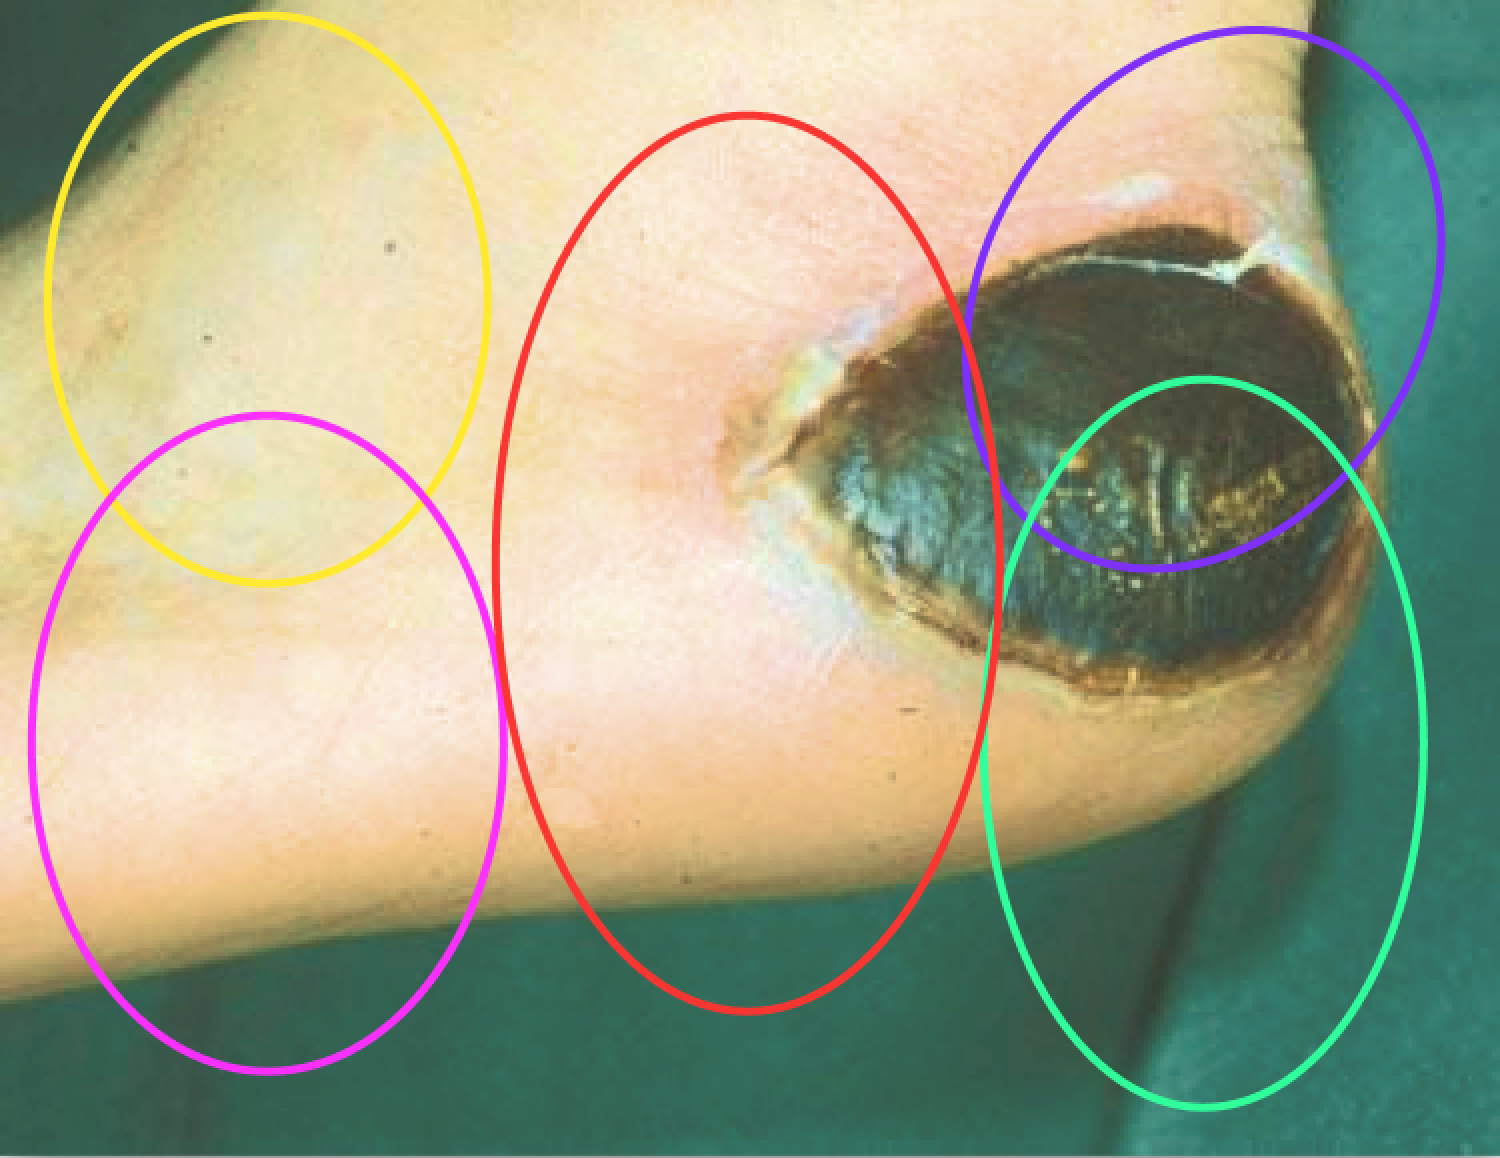
\includegraphics[width=\textwidth]{gambar/gambar-3_7.png}
% 		\caption{}
% 	\end{subfigure} 
% 	\caption{
% 		(a) Citra gambar luka, (b) Deteksi \emph{clustering} citra dengan GMM
% 	}
% \end{figure}

\subsection{Mempelajari parameter GMM}

Tahapan mempelajari parameter GMM dalam algoritma \emph{GrabCut} adalah untuk 
menghasilkan model yang akurat dalam memodelkan distribusi warna dari objek 
dan latar belakang dalam gambar. Tahap ini digunakan untuk memperbarui parameter-parameter 
GMM berdasarkan probabilitas posteriori. Algoritma menggunakan probabilitas posteriori 
piksel sebagai bobot dalam perhitungan rata-rata dan kovariansi baru untuk setiap 
komponen GMM. Dengan demikian, piksel yang memiliki probabilitas posteriori yang 
lebih tinggi akan memberikan kontribusi yang lebih besar dalam perhitungan parameter GMM.

Langkah dalam memperbarui parameter GMM dilakukan dengan langkah-langkah sebagai berikut:
\begin{enumerate}
    \item Untuk setiap komponen GMM dalam model objek dan latar belakang, hitung 
    rata-rata baru. Rata-rata baru dihitung dengan menggunakan probabilitas posteriori 
    piksel sebagai bobot dalam perhitungan rata-rata.
    \item Selanjutnya, perbarui kovariansi baru untuk setiap komponen GMM. Perhitungan 
    kovariansi baru juga menggunakan probabilitas posteriori sebagai bobot dalam 
    perhitungan kovariansi.
    \item Setelah perhitungan rata-rata dan kovariansi baru selesai untuk semua 
    komponen GMM, model GMM telah diperbarui.
\end{enumerate}

Dengan memperbarui parameter-parameter GMM berdasarkan probabilitas posteriori yang 
dihitung, algoritma secara bertahap meningkatkan model GMM agar sesuai dengan data gambar. 
Model yang lebih akurat membantu algoritma dalam membedakan antara piksel objek dan 
latar belakang, sehingga memperbaiki hasil segmentasi dengan lebih baik.


\subsection{Segmentasi Citra dengan Algoritma \emph{Mincut}}

Selanjutnya penulis melakukan segmentasi dengan menggunakan algoritma \emph{min-cut}
atau \emph{GraphCut}. Algoritma ini memvisualisasikan gambar sebagai graf, dan piksel 
sebagai \emph{node} pada graf tersebut, kemudian \emph{GraphCut} bertugas untuk 
segmentasi piksel mana yang termasuk \emph{foreground} dan \emph{background} dengan cara
melakukan \emph{cut} pada graf. Terdapat dua terminal pada graf yaitu terminal \emph{source} s
dan \emph{sink} t, kedua terminal saling terhubung terhadap semua piksel yang ada di graf,
piksel yang masuk ke dalam \emph{source} akan menjadi \emph{foreground} sementara piksel
yang masuk ke dalam \emph{sink} akan menjadi \emph{background}. Setiap \emph{node} 
pada graf memiliki hubungan yang yang disebut \emph{edge}, \emph{edge} akan memiliki arah 
dan bobot dimana bobot tersebut akan digunakan untuk mencari \emph{mincut} dari graf.


\begin{figure}[H]
	\centering
	  \begin{subfigure}{.5\textwidth}
		\centering{}
		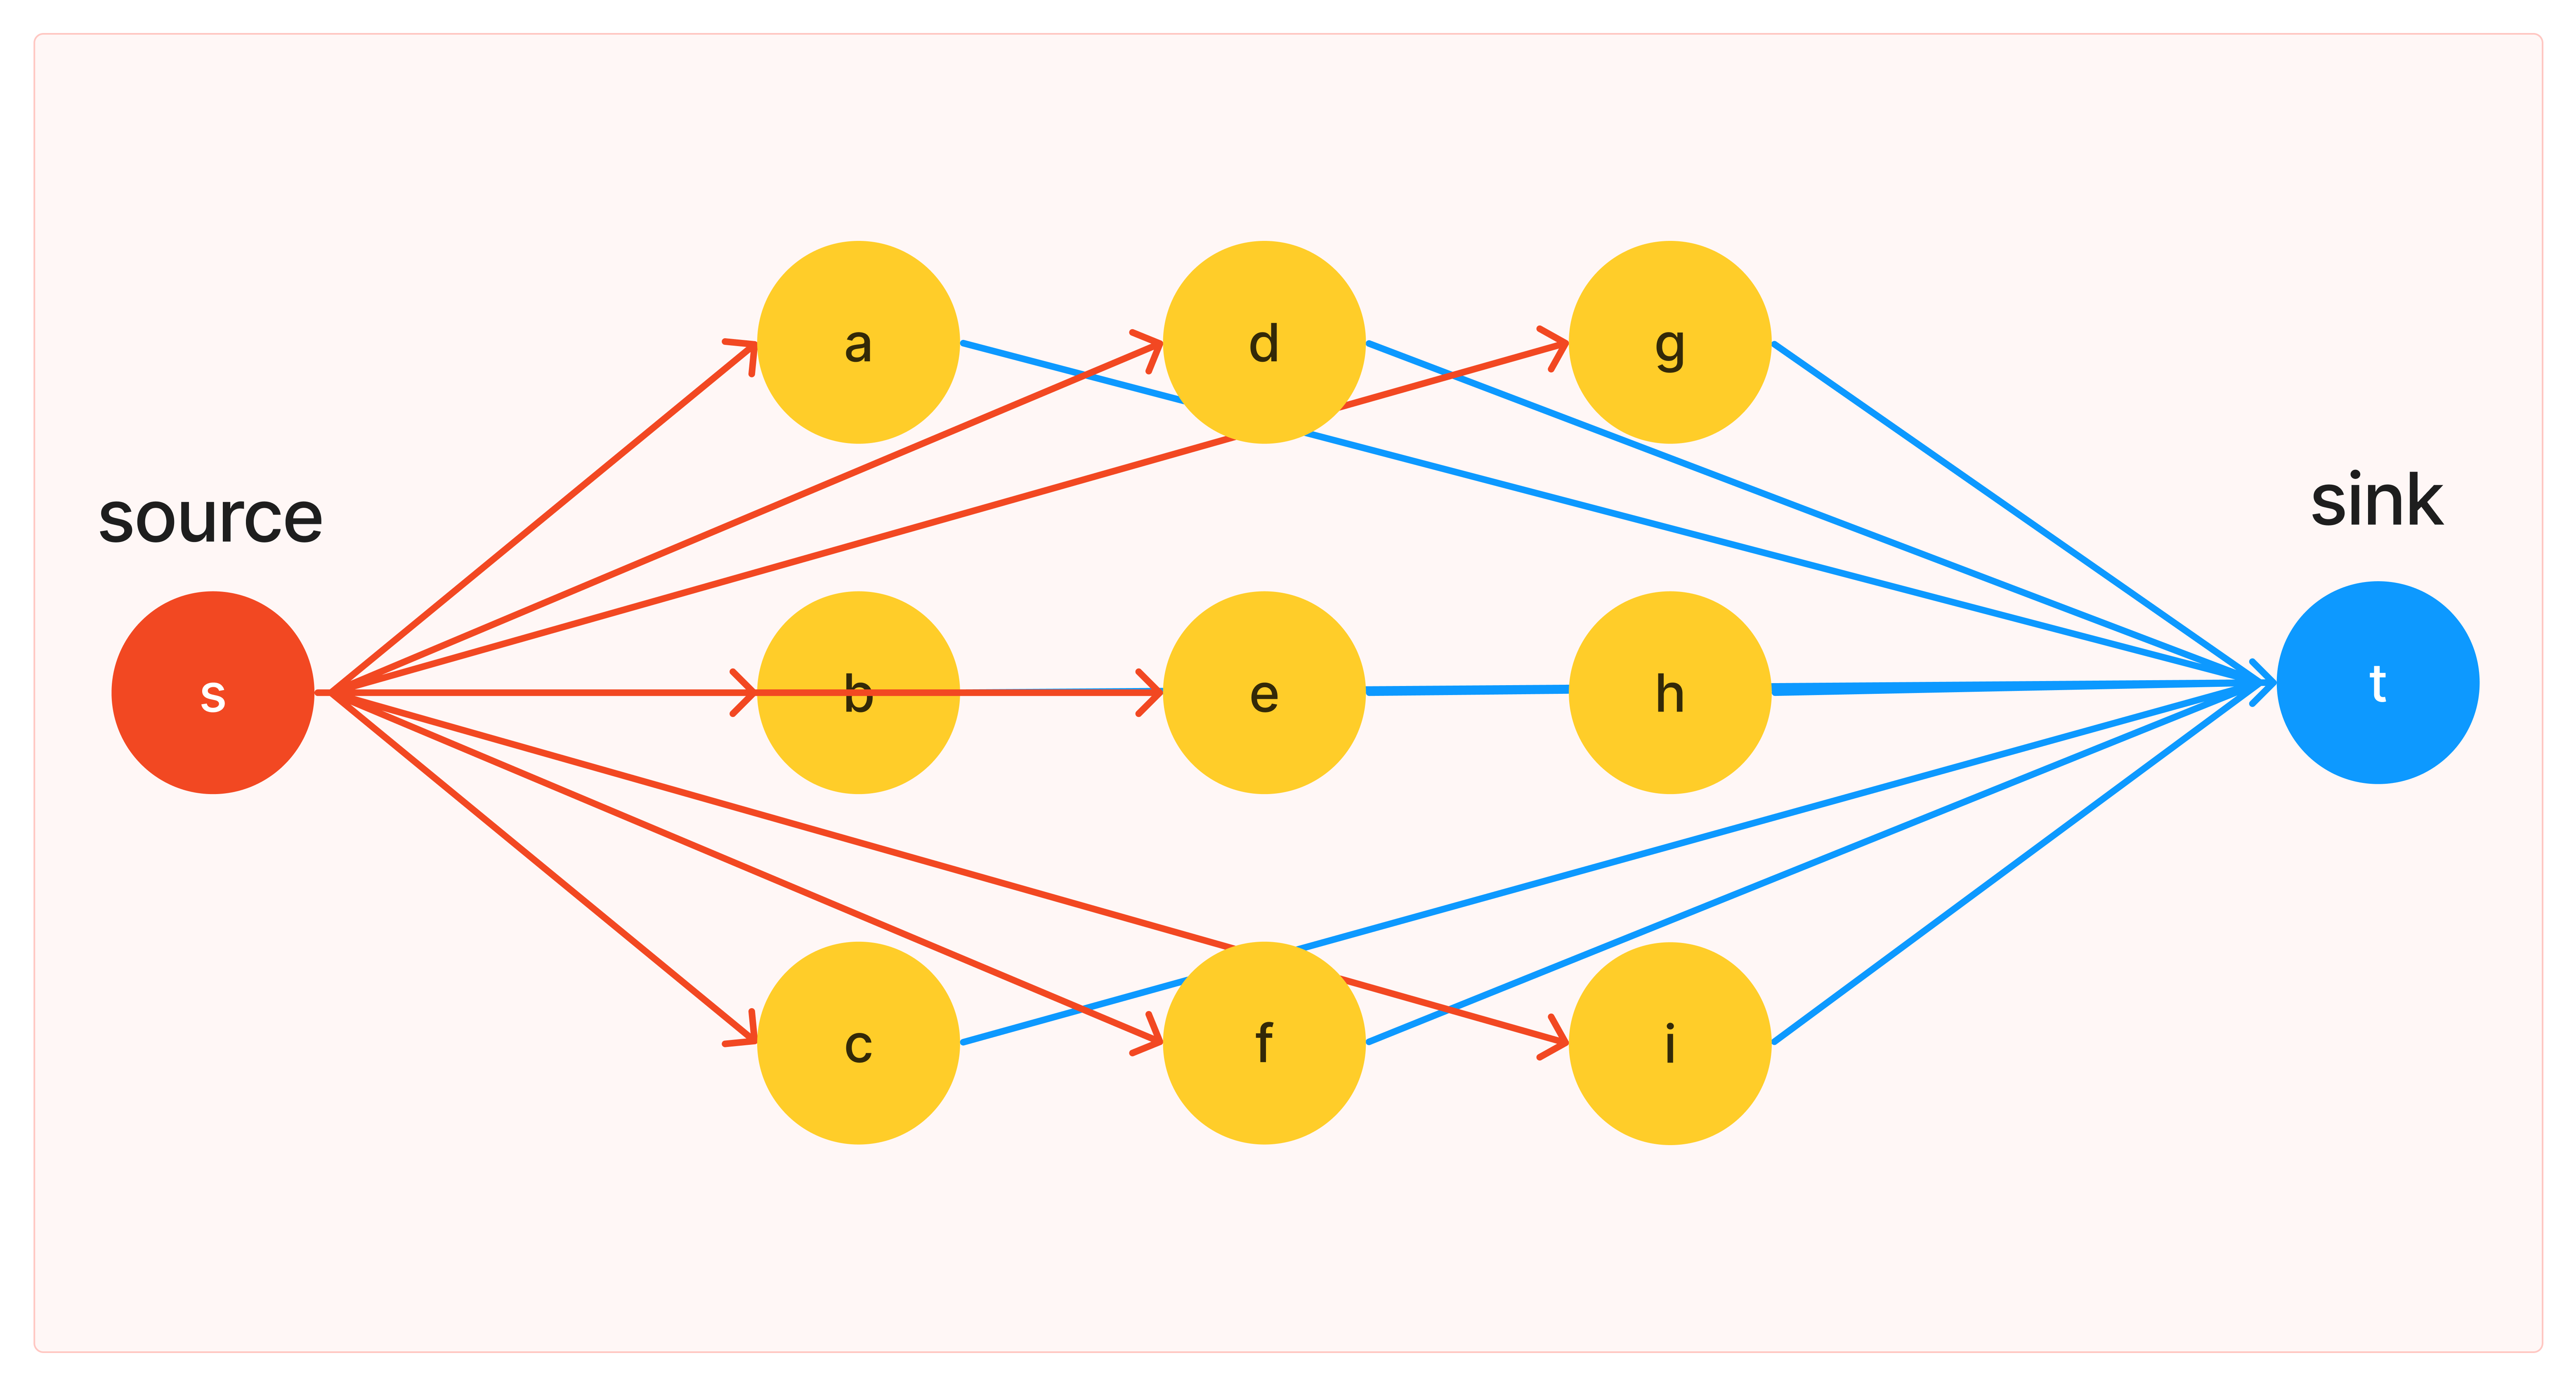
\includegraphics[width=\textwidth]{gambar/cth-graph-1.png}
		\caption{Sebuah graf}
	  \end{subfigure} \hfill
	  \begin{subfigure}{.5\textwidth}
		\centering{}
		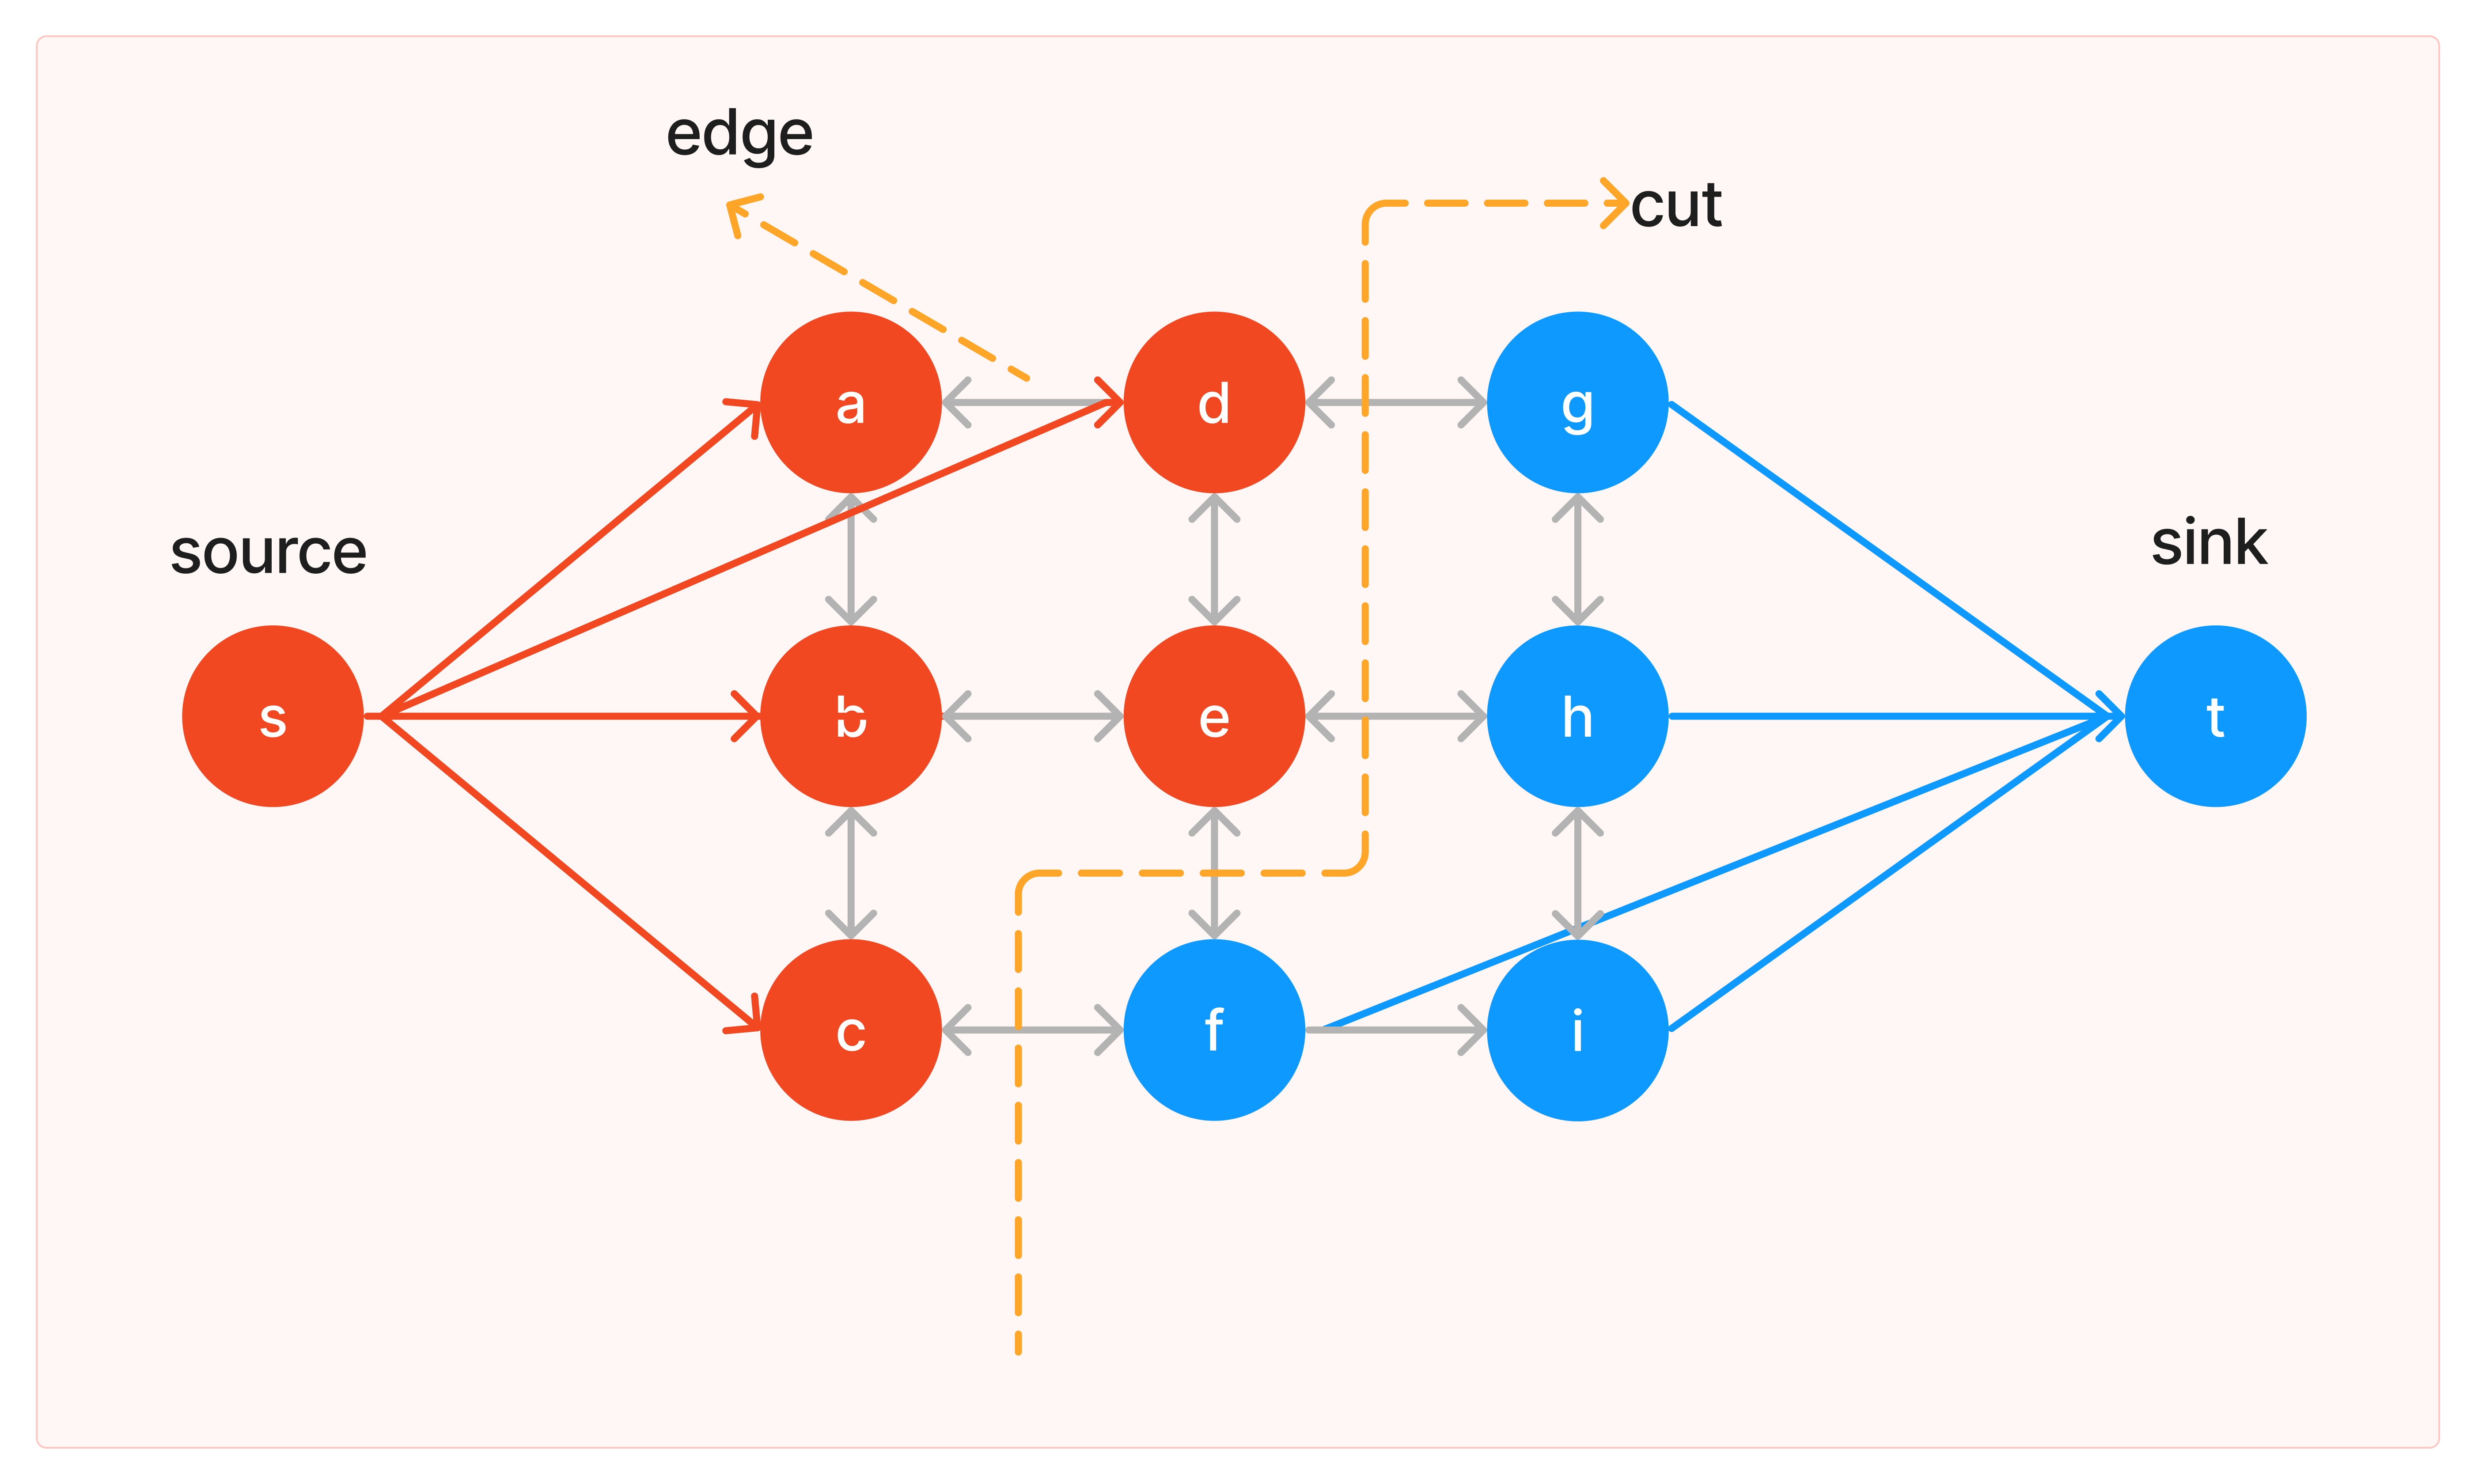
\includegraphics[width=\textwidth]{gambar/cth-graph-2.png}
		\caption{Sebuah (\emph{cut})}
	  \end{subfigure}  
	\caption{
	  Contoh graf berkapasitas terarah.
	  }
	\label{img:contoh_mincut}
  
  \end{figure}

Algoritma \emph{mincut} terdiri dari beberapa tahap, penjelasan singkatnya yaitu 
tahap pertama dimana graf bertumbuh (\emph{growth}) hingga menemukan jalan (\emph{path}) 
dari \emph{source} menuju \emph{sink}, selanjutnya tahap kedua (augmentasi) dimana 
\emph{path} yang sudah ditemukan akan dilihat kapasitas tiap \emph{edge} nya lalu 
masing-masing kapasitas \emph{edge} akan dikurangi dengan kapasitas paling kecil 
(\emph{bottleneck}), apabila ada kapasitas \emph{edge} yang kosong, maka \emph{node} 
tersebut menjadi \emph{Orphans} (tidak memiliki orang tua), setelah itu masuk tahap 
ketiga (adopsi) yaitu mencari orang tua baru dari \emph{node} yang menjadi \emph{orphans} 
sebelumnya, apabila tidak ada maka \emph{node} tersebut menjadi \emph{node} bebas. 
Struktur algoritma \emph{mincut} dapat dilihat pada bagian \ref{pseudo:1.0}. 

Setiap piksel pada gambar memiliki komponen GMM tersendiri, pada tahap ini nilai k
tiap piksel telah didapatkan dari GMM, dimana nilai k dari tiap piksel memiliki rentang
dari 1 sampai 5. Pada permulaan algoritma \emph{mincut} penulis menentukan \emph{node}
mana yang menjadi tetangga dari \emph{source} atau \emph{sink} dengan menghitung
menghitung jumlah nilai D dari persamaan \ref{eq:rumus_energi2} pada setiap komponen GMM, 
kemudian penulis menjumlahkan nilai yang didapat dan membaginya dengan 5 (total K),
nilai yang didapat akan dijadikan sebagai \emph{treshold} dalam menentukan hubungan
tiap piksel ke \emph{Source} atau ke \emph{Sink}. Tahap ini mensegmentasi citra 
yang telah dihitung setiap komponen pikselnya pada langkah-langkah sebelumnya sesuai 
dengan persamaan \ref{eq:rumus_energi1}.

% \begin{lstlisting} [label={pseudo: neighbors_terminals}]
% 	initialize: (P = [[], [], [], [], []], 
% 	S = [0,0,0,0,0], 
% 	G = (V, E), K = Himpunan komponen GMM tiap piksel)
% 	t = 0
% 	for every node x $\in$ V : 
% 		P[K[x]-1] := P[K[x]-1] $\cup$ {x}
% 		Calculate D for x using $\ref{eq:2.12}$
% 		S[K[x]-1] += D
% 	end for

% 	Calculate t := mean(S)

% 	for every k $\in$ {1,2,3,4,5}:
% 	if S[k-1] < t
% 		E := E $\cup$ (s $\rightarrow$ p) for every p $\in$ P[k-1]
% 	else
% 		E := E $\cup$ (p $\rightarrow$ t) for every p $\in$ P[k-1]
% 	end for

	
%   \end{lstlisting}

% Selanjutnya masuk ke tahap growth, \emph{augmentation}, dan \emph{adoption}, diagram alir
% dari ketiga tahap bisa dilihat sebagai berikut :

% dengan meminimumkan rumus E pada persamaan \ref{eq:2.10}, lalu kembali
% ke langkah awal sampai terjadinya konvergensi yaitu tidak ada perbedaan segmentasi antar Iterasi.

\subsection{Penyuntingan oleh Pengguna}
Langkah selanjutnya penulis melakukan perbaikan dari citra yang telah tersegmentasi
dari hasil sebelumnya, pengguna menggunakan \emph{brush} yaitu menggambar manual daerah 
yang menjadi \emph{background} dengan warna hitam, dan daerah objek dengan warna putih
kemudian melakukan algoritma \emph{mincut} yang hanya dilakukan sekali. Berikut 
gambaran simulasi penelitian yang akan penulis lakukan terhadap citra gambar luka 
untuk mendapatkan hasil segmentasi dengan metode \emph{GrabCut}:

\begin{figure}[H]
	\centering
	  \begin{subfigure}{0.3\textwidth}
		\centering{}
		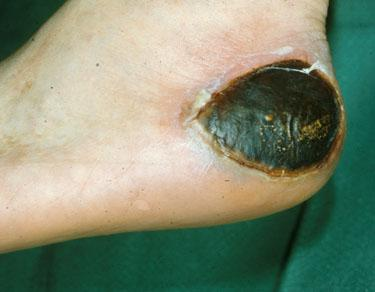
\includegraphics[width=\textwidth]{gambar/gambar-3_2(b).jpg}
		\caption{}
	  \end{subfigure}  
	  \begin{subfigure}{0.3\textwidth}
		\centering{}
		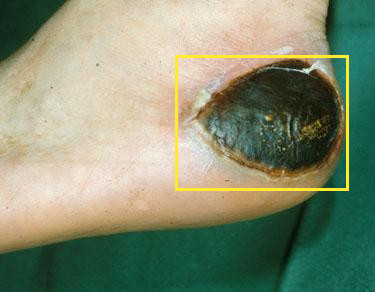
\includegraphics[width=\textwidth]{gambar/rectangle.png}
		\caption{}
	  \end{subfigure}
      \begin{subfigure}{0.3\textwidth}
		\centering{}
		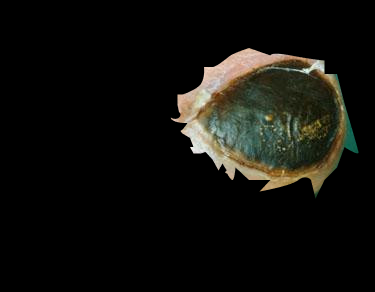
\includegraphics[width=\textwidth]{gambar/res_1.png}
		\caption{}
	  \end{subfigure}
      \begin{subfigure}{0.3\textwidth}
		\centering{}
		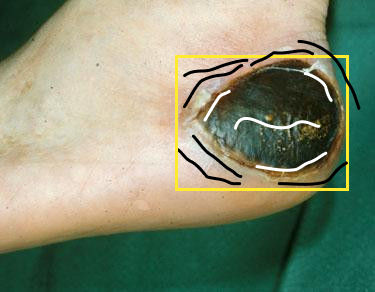
\includegraphics[width=\textwidth]{gambar/brush.png}
		\caption{}
	  \end{subfigure}
      \begin{subfigure}{0.3\textwidth}
		\centering{}
		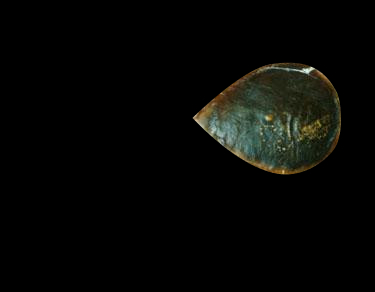
\includegraphics[width=\textwidth]{gambar/res_2.png}
		\caption{}
	  \end{subfigure}
	\caption{
		(a) Data citra luka 2.png, (b) \emph{Bounding box} area luka, (c) Hasil 
        segmentasi \emph{GrabCut} sebelum diperbaiki, (d) Penyuntingan manual oleh pengguna, (e) Hasil akhir setelah diperbaiki
	 }
  \end{figure}

\subsection{Menghitung Tingkat Akurasi}
Untuk menemukan nilai hasil segmentasi citra luka dengan menggunakan algoritma \emph{GrabCut},
yaitu mencari nilai akurasi citra, dengan menghitung selisih piksel dari area
segmentasi dengan area citra referensi sehingga akan menghasilkan nilai akurasi berikut :
\begin{equation} \label{eq:validasi}
	Akurasi(\%) = 100 - \bigg | \frac{(luas \: area \: citra \: referensi - luas \: area \: segmentasi)}{luas \: area \: citra \: referensi} * 100 \bigg |
\end{equation}.


\section{Skenario Eksperimen} \label{section:skenario_eksperimen}

Berikut adalah skenario eksperimen untuk "Deteksi Area Keliling Luka Kronis 
Menggunakan \emph{GRABCUT}"

\begin{enumerate}
    \item{Input gambar luka kronis}
    \item{Pengguna memberi kotak pembatas di sekeliling area luka (objek) pada gambar luka}
    \item{Inisiasi titik koordinat \((y,x)\) kotak pembatas di dalam gambar luka}
    \item{Memberi penanda area di luar kotak dengan angka 1, dan area di luar kotak
    dengan angka 0}
    \item{Memasukkan komponen GMM di setiap piksel untuk menghitung probabilitas 
    tiap piksel }
    \item{Mempelajari parameter GMM dengan melihat hasil probabilitas objek atau latar belakang}
    \item{Segmentasi area keliling luka dengan menggunakan algoritma \emph{GraphCut}}
    \item{Ulangi sampai sesuai dengan area luka}
    \item{Pengguna mengedit bagian mana yang menjadi objek dan latar belakang 
    dengan menggunaan \emph{Brush Tools} setelah itu jalankan tahap 7 satu kali  }
    \item{Mendapatkan Nilai \emph{Image Similarity}}
  \end{enumerate}